%%%%%%%%%%%%%%%%%%%%%%%%%%%%%%%%%%%%%%%%%
% The Legrand Orange Book
% LaTeX Template
% Version 2.3 (8/8/17)
%
% This template has been downloaded from:
% http://www.LaTeXTemplates.com
%
% Original author:
% Mathias Legrand (legrand.mathias@gmail.com) with modifications by:
% Vel (vel@latextemplates.com)
%
% License:
% CC BY-NC-SA 3.0 (http://creativecommons.org/licenses/by-nc-sa/3.0/)
%
% Compiling this template:
% This template uses biber for its bibliography and makeindex for its index.
% When you first open the template, compile it from the command line with the
% commands below to make sure your LaTeX distribution is configured correctly:
%
% 1) pdflatex main
% 2) makeindex main.idx -s StyleInd.ist
% 3) biber main
% 4) pdflatex main x 2
%
% After this, when you wish to update the bibliography/index use the appropriate
% command above and make sure to compile with pdflatex several times
% afterwards to propagate your changes to the document.
%
% This template also uses a number of packages which may need to be
% updated to the newest versions for the template to compile. It is strongly
% recommended you update your LaTeX distribution if you have any
% compilation errors.
%
% Important note:
% Chapter heading images should have a 2:1 width:height ratio,
% e.g. 920px width and 460px height.
%
%%%%%%%%%%%%%%%%%%%%%%%%%%%%%%%%%%%%%%%%%

%----------------------------------------------------------------------------------------
%	PACKAGES AND OTHER DOCUMENT CONFIGURATIONS
%----------------------------------------------------------------------------------------

\documentclass[11pt,fleqn]{book} % Default font size and left-justified equations
% \documentclass[11pt,fleqn]{ctexbook} % Default font size and left-justified equations

%----------------------------------------------------------------------------------------
\usepackage{fontspec}
\usepackage[UTF8]{ctex}
\usepackage{xeCJK}
\setmainfont{Times}
\setCJKmainfont{Songti TC}
% \setCJKmainfont{Xingkai TC}
%%%%%%%%%%%%%%%%%%%%%%%%%%%%%%%%%%%%%%%%%
% The Legrand Orange Book
% Structural Definitions File
% Version 2.0 (9/2/15)
%
% Original author:
% Mathias Legrand (legrand.mathias@gmail.com) with modifications by:
% Vel (vel@latextemplates.com)
% 
% This file has been downloaded from:
% http://www.LaTeXTemplates.com
%
% License:
% CC BY-NC-SA 3.0 (http://creativecommons.org/licenses/by-nc-sa/3.0/)
%
%%%%%%%%%%%%%%%%%%%%%%%%%%%%%%%%%%%%%%%%%

%----------------------------------------------------------------------------------------
%	VARIOUS REQUIRED PACKAGES AND CONFIGURATIONS
%----------------------------------------------------------------------------------------

\usepackage[top=3cm,bottom=3cm,left=3cm,right=3cm,headsep=10pt,a4paper]{geometry} % Page margins

\usepackage{graphicx} % Required for including pictures
\graphicspath{{Pictures/}} % Specifies the directory where pictures are stored

\usepackage{lipsum} % Inserts dummy text

\usepackage{tikz} % Required for drawing custom shapes

\usepackage[english]{babel} % English language/hyphenation

\usepackage{enumitem} % Customize lists
\setlist{nolistsep} % Reduce spacing between bullet points and numbered lists

\usepackage{booktabs} % Required for nicer horizontal rules in tables

\usepackage{xcolor} % Required for specifying colors by name
\definecolor{ocre}{RGB}{243,102,25} % Define the orange color used for highlighting throughout the book

%----------------------------------------------------------------------------------------
%	FONTS
%----------------------------------------------------------------------------------------

\usepackage{avant} % Use the Avantgarde font for headings
%\usepackage{times} % Use the Times font for headings
\usepackage{mathptmx} % Use the Adobe Times Roman as the default text font together with math symbols from the Sym­bol, Chancery and Com­puter Modern fonts

\usepackage{microtype} % Slightly tweak font spacing for aesthetics
\usepackage[utf8]{inputenc} % Required for including letters with accents
\usepackage[T1]{fontenc} % Use 8-bit encoding that has 256 glyphs

%----------------------------------------------------------------------------------------
%	BIBLIOGRAPHY AND INDEX
%----------------------------------------------------------------------------------------

\usepackage[style=numeric,citestyle=numeric,sorting=nyt,sortcites=true,autopunct=true,babel=hyphen,hyperref=true,abbreviate=false,backref=true,backend=biber]{biblatex}
\addbibresource{bibliography.bib} % BibTeX bibliography file
\defbibheading{bibempty}{}

\usepackage{calc} % For simpler calculation - used for spacing the index letter headings correctly
\usepackage{makeidx} % Required to make an index
\makeindex % Tells LaTeX to create the files required for indexing

%----------------------------------------------------------------------------------------
%	MAIN TABLE OF CONTENTS
%----------------------------------------------------------------------------------------

\usepackage{titletoc} % Required for manipulating the table of contents

\contentsmargin{0cm} % Removes the default margin

% Part text styling
\titlecontents{part}[0cm]
{\addvspace{20pt}\centering\large\bfseries}
{}
{}
{}

% Chapter text styling
\titlecontents{chapter}[1.25cm] % Indentation
{\addvspace{12pt}\large\bfseries} % Spacing and font options for chapters
{\color{ocre!60}\contentslabel[\Large\thecontentslabel]{1.25cm}\color{ocre}} % Chapter number
{\color{ocre}}  
{\color{ocre!60}\normalsize\;\titlerule*[.5pc]{.}\;\thecontentspage} % Page number

% Section text styling
\titlecontents{section}[1.25cm] % Indentation
{\addvspace{3pt}\bfseries} % Spacing and font options for sections
{\contentslabel[\thecontentslabel]{1.25cm}} % Section number
{}
{\hfill\color{black}\thecontentspage} % Page number
[]

% Subsection text styling
\titlecontents{subsection}[1.25cm] % Indentation
{\addvspace{1pt}\small} % Spacing and font options for subsections
{\contentslabel[\thecontentslabel]{1.25cm}} % Subsection number
{}
{\ \titlerule*[.5pc]{.}\;\thecontentspage} % Page number
[]

% List of figures
\titlecontents{figure}[0em]
{\addvspace{-5pt}}
{\thecontentslabel\hspace*{1em}}
{}
{\ \titlerule*[.5pc]{.}\;\thecontentspage}
[]

% List of tables
\titlecontents{table}[0em]
{\addvspace{-5pt}}
{\thecontentslabel\hspace*{1em}}
{}
{\ \titlerule*[.5pc]{.}\;\thecontentspage}
[]

%----------------------------------------------------------------------------------------
%	MINI TABLE OF CONTENTS IN PART HEADS
%----------------------------------------------------------------------------------------

% Chapter text styling
\titlecontents{lchapter}[0em] % Indenting
{\addvspace{15pt}\large\bfseries} % Spacing and font options for chapters
{\color{ocre}\contentslabel[\Large\thecontentslabel]{1.25cm}\color{ocre}} % Chapter number
{}  
{\color{ocre}\normalsize\bfseries\;\titlerule*[.5pc]{.}\;\thecontentspage} % Page number

% Section text styling
\titlecontents{lsection}[0em] % Indenting
{\small} % Spacing and font options for sections
{\contentslabel[\thecontentslabel]{1.25cm}} % Section number
{}
{}

% Subsection text styling
\titlecontents{lsubsection}[.5em] % Indentation
{\normalfont\footnotesize} % Font settings
{}
{}
{}

%----------------------------------------------------------------------------------------
%	PAGE HEADERS
%----------------------------------------------------------------------------------------

\usepackage{fancyhdr} % Required for header and footer configuration

\pagestyle{fancy}
\renewcommand{\chaptermark}[1]{\markboth{\normalsize\bfseries\chaptername\ \thechapter.\ #1}{}} % Chapter text font settings
\renewcommand{\sectionmark}[1]{\markright{\normalsize\thesection\hspace{5pt}#1}{}} % Section text font settings
\fancyhf{} \fancyhead[LE,RO]{\normalsize\thepage} % Font setting for the page number in the header
\fancyhead[LO]{\rightmark} % Print the nearest section name on the left side of odd pages
\fancyhead[RE]{\leftmark} % Print the current chapter name on the right side of even pages
\renewcommand{\headrulewidth}{0.5pt} % Width of the rule under the header
\addtolength{\headheight}{2.5pt} % Increase the spacing around the header slightly
\renewcommand{\footrulewidth}{0pt} % Removes the rule in the footer
\fancypagestyle{plain}{\fancyhead{}\renewcommand{\headrulewidth}{0pt}} % Style for when a plain pagestyle is specified

% Removes the header from odd empty pages at the end of chapters
\makeatletter
\renewcommand{\cleardoublepage}{
\clearpage\ifodd\c@page\else
\hbox{}
\vspace*{\fill}
\thispagestyle{empty}
% \newpage
\fi}

%----------------------------------------------------------------------------------------
%	THEOREM STYLES
%----------------------------------------------------------------------------------------

\usepackage{amsmath,amsfonts,amssymb,amsthm} % For math equations, theorems, symbols, etc

\newcommand{\intoo}[2]{\mathopen{]}#1\,;#2\mathclose{[}}
\newcommand{\ud}{\mathop{\mathrm{{}d}}\mathopen{}}
\newcommand{\intff}[2]{\mathopen{[}#1\,;#2\mathclose{]}}
\newtheorem{notation}{Notation}[chapter]

% Boxed/framed environments
\newtheoremstyle{ocrenumbox}% % Theorem style name
{0pt}% Space above
{0pt}% Space below
{\normalfont}% % Body font
{}% Indent amount
{\small\bf\color{ocre}}% % Theorem head font
{\;}% Punctuation after theorem head
{0.25em}% Space after theorem head
{\small\color{ocre}\thmname{#1}\nobreakspace\thmnumber{\@ifnotempty{#1}{}\@upn{#2}}% Theorem text (e.g. Theorem 2.1)
\thmnote{\nobreakspace\the\thm@notefont\bfseries\color{black}---\nobreakspace#3.}} % Optional theorem note
\renewcommand{\qedsymbol}{$\blacksquare$}% Optional qed square

\newtheoremstyle{blacknumex}% Theorem style name
{5pt}% Space above
{5pt}% Space below
{\normalfont}% Body font
{} % Indent amount
{\small\bf}% Theorem head font
{\;}% Punctuation after theorem head
{0.25em}% Space after theorem head
{\small{\tiny\ensuremath{\blacksquare}}\nobreakspace\thmname{#1}\nobreakspace\thmnumber{\@ifnotempty{#1}{}\@upn{#2}}% Theorem text (e.g. Theorem 2.1)
\thmnote{\nobreakspace\the\thm@notefont\bfseries---\nobreakspace#3.}}% Optional theorem note

\newtheoremstyle{blacknumbox} % Theorem style name
{0pt}% Space above
{0pt}% Space below
{\normalfont}% Body font
{}% Indent amount
{\small\bf}% Theorem head font
{\;}% Punctuation after theorem head
{0.25em}% Space after theorem head
{\small\thmname{#1}\nobreakspace\thmnumber{\@ifnotempty{#1}{}\@upn{#2}}% Theorem text (e.g. Theorem 2.1)
\thmnote{\nobreakspace\the\thm@notefont\bfseries---\nobreakspace#3.}}% Optional theorem note

% Non-boxed/non-framed environments
\newtheoremstyle{ocrenum}% % Theorem style name
{5pt}% Space above
{5pt}% Space below
{\normalfont}% % Body font
{}% Indent amount
{\small\bf\color{ocre}}% % Theorem head font
{\;}% Punctuation after theorem head
{0.25em}% Space after theorem head
{\small\color{ocre}\thmname{#1}\nobreakspace\thmnumber{\@ifnotempty{#1}{}\@upn{#2}}% Theorem text (e.g. Theorem 2.1)
\thmnote{\nobreakspace\the\thm@notefont\bfseries\color{black}---\nobreakspace#3.}} % Optional theorem note
\renewcommand{\qedsymbol}{$\blacksquare$}% Optional qed square
\makeatother

% Defines the theorem text style for each type of theorem to one of the three styles above
\newcounter{dummy} 
\numberwithin{dummy}{section}
\theoremstyle{ocrenumbox}
\newtheorem{theoremeT}[dummy]{Theorem}
\newtheorem{problem}{Problem}[chapter]
\newtheorem{exerciseT}{Exercise}[chapter]
\theoremstyle{blacknumex}
\newtheorem{exampleT}{Example}[chapter]
\theoremstyle{blacknumbox}
\newtheorem{vocabulary}{Vocabulary}[chapter]
\newtheorem{definitionT}{Definition}[section]
\newtheorem{corollaryT}[dummy]{Corollary}
\theoremstyle{ocrenum}
\newtheorem{proposition}[dummy]{Proposition}

%----------------------------------------------------------------------------------------
%	DEFINITION OF COLORED BOXES
%----------------------------------------------------------------------------------------

\RequirePackage[framemethod=default]{mdframed} % Required for creating the theorem, definition, exercise and corollary boxes

% Theorem box
\newmdenv[skipabove=7pt,
skipbelow=7pt,
backgroundcolor=black!5,
linecolor=ocre,
innerleftmargin=5pt,
innerrightmargin=5pt,
innertopmargin=5pt,
leftmargin=0cm,
rightmargin=0cm,
innerbottommargin=5pt]{tBox}

% Exercise box	  
\newmdenv[skipabove=7pt,
skipbelow=7pt,
rightline=false,
leftline=true,
topline=false,
bottomline=false,
backgroundcolor=ocre!10,
linecolor=ocre,
innerleftmargin=5pt,
innerrightmargin=5pt,
innertopmargin=5pt,
innerbottommargin=5pt,
leftmargin=0cm,
rightmargin=0cm,
linewidth=4pt]{eBox}	

% Definition box
\newmdenv[skipabove=7pt,
skipbelow=7pt,
rightline=false,
leftline=true,
topline=false,
bottomline=false,
linecolor=ocre,
innerleftmargin=5pt,
innerrightmargin=5pt,
innertopmargin=0pt,
leftmargin=0cm,
rightmargin=0cm,
linewidth=4pt,
innerbottommargin=0pt]{dBox}	

% Corollary box
\newmdenv[skipabove=7pt,
skipbelow=7pt,
rightline=false,
leftline=true,
topline=false,
bottomline=false,
linecolor=gray,
backgroundcolor=black!5,
innerleftmargin=5pt,
innerrightmargin=5pt,
innertopmargin=5pt,
leftmargin=0cm,
rightmargin=0cm,
linewidth=4pt,
innerbottommargin=5pt]{cBox}

% Creates an environment for each type of theorem and assigns it a theorem text style from the "Theorem Styles" section above and a colored box from above
\newenvironment{theorem}{\begin{tBox}\begin{theoremeT}}{\end{theoremeT}\end{tBox}}
\newenvironment{exercise}{\begin{eBox}\begin{exerciseT}}{\hfill{\color{ocre}\tiny\ensuremath{\blacksquare}}\end{exerciseT}\end{eBox}}				  
\newenvironment{definition}{\begin{dBox}\begin{definitionT}}{\end{definitionT}\end{dBox}}	
\newenvironment{example}{\begin{exampleT}}{\hfill{\tiny\ensuremath{\blacksquare}}\end{exampleT}}		
\newenvironment{corollary}{\begin{cBox}\begin{corollaryT}}{\end{corollaryT}\end{cBox}}	

%----------------------------------------------------------------------------------------
%	REMARK ENVIRONMENT
%----------------------------------------------------------------------------------------

\newenvironment{remark}{\par\vspace{10pt}\small % Vertical white space above the remark and smaller font size
\begin{list}{}{
\leftmargin=35pt % Indentation on the left
\rightmargin=25pt}\item\ignorespaces % Indentation on the right
\makebox[-2.5pt]{\begin{tikzpicture}[overlay]
\node[draw=ocre!60,line width=1pt,circle,fill=ocre!25,font=\bfseries,inner sep=2pt,outer sep=0pt] at (-15pt,0pt){\textcolor{ocre}{R}};\end{tikzpicture}} % Orange R in a circle
\advance\baselineskip -1pt}{\end{list}\vskip5pt} % Tighter line spacing and white space after remark

%----------------------------------------------------------------------------------------
%	SECTION NUMBERING IN THE MARGIN
%----------------------------------------------------------------------------------------

\makeatletter
\renewcommand{\@seccntformat}[1]{\llap{\textcolor{ocre}{\csname the#1\endcsname}\hspace{1em}}}                    
\renewcommand{\section}{\@startsection{section}{1}{\z@}
{-4ex \@plus -1ex \@minus -.4ex}
{1ex \@plus.2ex }
{\normalfont\large\bfseries}}
\renewcommand{\subsection}{\@startsection {subsection}{2}{\z@}
{-3ex \@plus -0.1ex \@minus -.4ex}
{0.5ex \@plus.2ex }
{\normalfont\bfseries}}
\renewcommand{\subsubsection}{\@startsection {subsubsection}{3}{\z@}
{-2ex \@plus -0.1ex \@minus -.2ex}
{.2ex \@plus.2ex }
{\normalfont\small\bfseries}}                        
\renewcommand\paragraph{\@startsection{paragraph}{4}{\z@}
{-2ex \@plus-.2ex \@minus .2ex}
{.1ex}
{\normalfont\small\bfseries}}

%----------------------------------------------------------------------------------------
%	PART HEADINGS
%----------------------------------------------------------------------------------------

% numbered part in the table of contents
\newcommand{\@mypartnumtocformat}[2]{%
\setlength\fboxsep{0pt}%
\noindent\colorbox{ocre!20}{\strut\parbox[c][.7cm]{\ecart}{\color{ocre!70}\Large\bfseries\centering#1}}\hskip\esp\colorbox{ocre!40}{\strut\parbox[c][.7cm]{\linewidth-\ecart-\esp}{\Large\centering#2}}}%
%%%%%%%%%%%%%%%%%%%%%%%%%%%%%%%%%%
% unnumbered part in the table of contents
\newcommand{\@myparttocformat}[1]{%
\setlength\fboxsep{0pt}%
\noindent\colorbox{ocre!40}{\strut\parbox[c][.7cm]{\linewidth}{\Large\centering#1}}}%
%%%%%%%%%%%%%%%%%%%%%%%%%%%%%%%%%%
\newlength\esp
\setlength\esp{4pt}
\newlength\ecart
\setlength\ecart{1.2cm-\esp}
\newcommand{\thepartimage}{}%
\newcommand{\partimage}[1]{\renewcommand{\thepartimage}{#1}}%
\def\@part[#1]#2{%
\ifnum \c@secnumdepth >-2\relax%
\refstepcounter{part}%
\addcontentsline{toc}{part}{\texorpdfstring{\protect\@mypartnumtocformat{\thepart}{#1}}{\partname~\thepart\ ---\ #1}}
\else%
\addcontentsline{toc}{part}{\texorpdfstring{\protect\@myparttocformat{#1}}{#1}}%
\fi%
\startcontents%
\markboth{}{}%
{\thispagestyle{empty}%
\begin{tikzpicture}[remember picture,overlay]%
\node at (current page.north west){\begin{tikzpicture}[remember picture,overlay]%	
\fill[ocre!20](0cm,0cm) rectangle (\paperwidth,-\paperheight);
\node[anchor=north] at (4cm,-3.25cm){\color{ocre!40}\fontsize{220}{100}\bfseries\thepart}; 
\node[anchor=south east] at (\paperwidth-1cm,-\paperheight+1cm){\parbox[t][][t]{8.5cm}{
\printcontents{l}{0}{\setcounter{tocdepth}{1}}%
}};
\node[anchor=north east] at (\paperwidth-1.5cm,-3.25cm){\parbox[t][][t]{15cm}{\strut\raggedleft\color{white}\fontsize{30}{30}\bfseries#2}};
\end{tikzpicture}};
\end{tikzpicture}}%
\@endpart}
\def\@spart#1{%
\startcontents%
\phantomsection
{\thispagestyle{empty}%
\begin{tikzpicture}[remember picture,overlay]%
\node at (current page.north west){\begin{tikzpicture}[remember picture,overlay]%	
\fill[ocre!20](0cm,0cm) rectangle (\paperwidth,-\paperheight);
\node[anchor=north east] at (\paperwidth-1.5cm,-3.25cm){\parbox[t][][t]{15cm}{\strut\raggedleft\color{white}\fontsize{30}{30}\bfseries#1}};
\end{tikzpicture}};
\end{tikzpicture}}
\addcontentsline{toc}{part}{\texorpdfstring{%
\setlength\fboxsep{0pt}%
\noindent\protect\colorbox{ocre!40}{\strut\protect\parbox[c][.7cm]{\linewidth}{\Large\protect\centering #1\quad\mbox{}}}}{#1}}%
\@endpart}
\def\@endpart{\vfil
% \newpage
\if@twoside
\if@openright
\null
\thispagestyle{empty}%
% \newpage
\fi
\fi
\if@tempswa
\twocolumn
\fi}

%----------------------------------------------------------------------------------------
%	CHAPTER HEADINGS
%----------------------------------------------------------------------------------------

% A switch to conditionally include a picture, implemented by  Christian Hupfer
\newif\ifusechapterimage
\usechapterimagetrue
\newcommand{\thechapterimage}{}%
\newcommand{\chapterimage}[1]{\ifusechapterimage\renewcommand{\thechapterimage}{#1}\fi}%
\newcommand{\autodot}{.}
\def\@makechapterhead#1{%
{\parindent \z@ \raggedright \normalfont
\ifnum \c@secnumdepth >\m@ne
\if@mainmatter
\begin{tikzpicture}[remember picture,overlay]
\node at (current page.north west)
{\begin{tikzpicture}[remember picture,overlay]
\node[anchor=north west,inner sep=0pt] at (0,0) {\ifusechapterimage\includegraphics[width=\paperwidth]{\thechapterimage}\fi};
\draw[anchor=west] (\Gm@lmargin,-9cm) node [line width=2pt,rounded corners=15pt,draw=ocre,fill=white,fill opacity=0.5,inner sep=15pt]{\strut\makebox[22cm]{}};
\draw[anchor=west] (\Gm@lmargin+.3cm,-9cm) node {\huge\bfseries\color{black}\thechapter\autodot~#1\strut};
\end{tikzpicture}};
\end{tikzpicture}
\else
\begin{tikzpicture}[remember picture,overlay]
\node at (current page.north west)
{\begin{tikzpicture}[remember picture,overlay]
\node[anchor=north west,inner sep=0pt] at (0,0) {\ifusechapterimage\includegraphics[width=\paperwidth]{\thechapterimage}\fi};
\draw[anchor=west] (\Gm@lmargin,-9cm) node [line width=2pt,rounded corners=15pt,draw=ocre,fill=white,fill opacity=0.5,inner sep=15pt]{\strut\makebox[22cm]{}};
\draw[anchor=west] (\Gm@lmargin+.3cm,-9cm) node {\huge\bfseries\color{black}#1\strut};
\end{tikzpicture}};
\end{tikzpicture}
\fi\fi\par\vspace*{270\p@}}}

%-------------------------------------------

\def\@makeschapterhead#1{%
\begin{tikzpicture}[remember picture,overlay]
\node at (current page.north west)
{\begin{tikzpicture}[remember picture,overlay]
\node[anchor=north west,inner sep=0pt] at (0,0) {\ifusechapterimage\includegraphics[width=\paperwidth]{\thechapterimage}\fi};
\draw[anchor=west] (\Gm@lmargin,-9cm) node [line width=2pt,rounded corners=15pt,draw=ocre,fill=white,fill opacity=0.5,inner sep=15pt]{\strut\makebox[22cm]{}};
\draw[anchor=west] (\Gm@lmargin+.3cm,-9cm) node {\huge\bfseries\color{black}#1\strut};
\end{tikzpicture}};
\end{tikzpicture}
\par\vspace*{270\p@}}
\makeatother

%----------------------------------------------------------------------------------------
%	HYPERLINKS IN THE DOCUMENTS
%----------------------------------------------------------------------------------------

\usepackage{hyperref}
\hypersetup{hidelinks,backref=true,pagebackref=true,hyperindex=true,colorlinks=false,breaklinks=true,urlcolor= ocre,bookmarks=true,bookmarksopen=false,pdftitle={Title},pdfauthor={Author}}
\usepackage{bookmark}
\bookmarksetup{
open,
numbered,
addtohook={%
\ifnum\bookmarkget{level}=0 % chapter
\bookmarksetup{bold}%
\fi
\ifnum\bookmarkget{level}=-1 % part
\bookmarksetup{color=ocre,bold}%
\fi
}
}


% custom add package
\usepackage{fontspec}
\usepackage[UTF8]{ctex}
\usepackage{xeCJK}
\usepackage{verbatim}
\usepackage{lmodern}
\setmainfont{Times}
\setCJKmainfont{Songti TC}
% \setCJKmainfont{Xingkai TC} % Insert the commands.tex file which contains the majority of the structure behind the template

%\usepackage{ctexcap}
%\usepackage[heading]{ctex}
% \usepackage[UTF8]{ctex}
% \usepackage{xeCJK}
\usepackage{verbatim}
\usepackage{lmodern}
\begin{document}

%----------------------------------------------------------------------------------------
%	TITLE PAGE
%----------------------------------------------------------------------------------------

\begingroup
\thispagestyle{empty}
\begin{tikzpicture}[remember picture,overlay]
\node[inner sep=0pt] (background) at (current page.center) {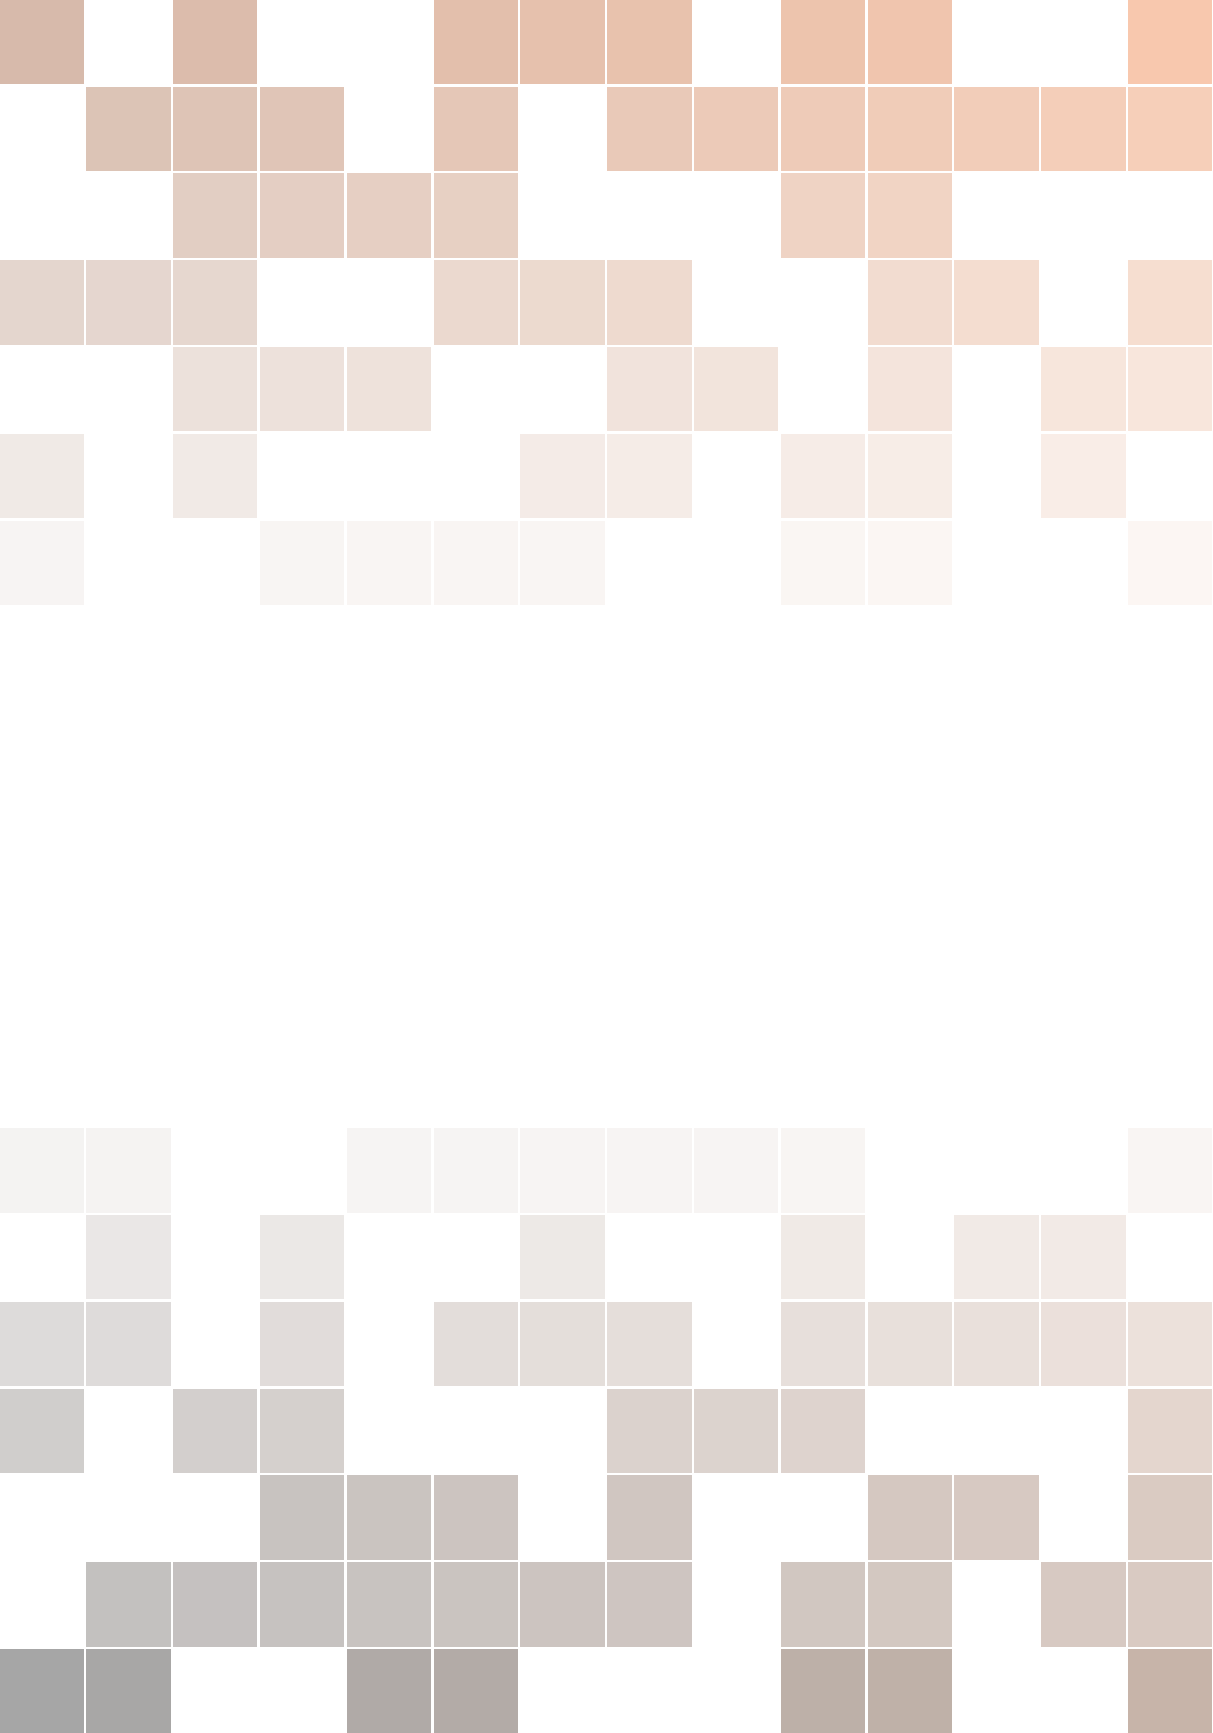
\includegraphics[width=\paperwidth]{background}};
\draw (current page.center) node [fill=ocre!30!white,fill opacity=0.6,text opacity=1,inner sep=1cm]
{
\Huge\centering\bfseries\parbox[c][][t]{\paperwidth}
% {\addvspace{12pt}\large\sffamily\bfseries} % Spacing and font options for chapters
 {\centering
 宇宙中不易被吹散的风\\[40pt] % Book title
% 文心雕龍\\[20pt] % Subtitle
 {\huge 采采流水}
 }
}; % Author name
\end{tikzpicture}
\vfill
\endgroup

%----------------------------------------------------------------------------------------
%	COPYRIGHT PAGE
%----------------------------------------------------------------------------------------

\newpage
~\vfill
\thispagestyle{empty}

\noindent Copyright \copyright\ 2013 John Smith\\ % Copyright notice

\noindent \textsc{Published by Publisher}\\ % Publisher

\noindent \textsc{book-website.com}\\ % URL

\noindent Licensed under the Creative Commons Attribution-NonCommercial 3.0 Unported License (the ``License''). You may not use this file except in compliance with the License. You may obtain a copy of the License at \url{http://creativecommons.org/licenses/by-nc/3.0}. Unless required by applicable law or agreed to in writing, software distributed under the License is distributed on an \textsc{``as is'' basis, without warranties or conditions of any kind}, either express or implied. See the License for the specific language governing permissions and limitations under the License.\\ % License information

\noindent \textit{First printing, March 2017} % Printing/edition date

%----------------------------------------------------------------------------------------
%	TABLE OF CONTENTS
%----------------------------------------------------------------------------------------

%\usechapterimagefalse % If you don't want to include a chapter image, use this to toggle images off - it can be enabled later with \usechapterimagetrue

\chapterimage{chapter_head_1.pdf} % Table of contents heading image

\pagestyle{empty} % No headers

\tableofcontents % Print the table of contents itself

% \cleardoublepage % Forces the first chapter to start on an odd page so it's on the right

\pagestyle{fancy} % Print headers again

%----------------------------------------------------------------------------------------
%	PART
%----------------------------------------------------------------------------------------

\part{Part One}

%----------------------------------------------------------------------------------------
%	CHAPTER 1
%----------------------------------------------------------------------------------------

\chapterimage{chapter_head_2.pdf} % Chapter heading image

%\chapter{Text Chapter}
\chapter{此情可待}

\section{ 伶官传序}

呜呼!盛衰之理,虽曰天命,岂非人事哉!原庄宗之所以得天下,与其所以失之者,可以知之矣。

世言晋王之将终也,以三矢赐庄宗而告之曰:“梁,吾仇也;燕王,吾所立,契丹与吾约为兄弟,而皆背晋以归梁。此三者,吾遗恨也。与尔三矢,尔其无忘乃父之志!”庄宗受而藏之于庙。其后用兵,则遣从事以一少牢告庙,请其矢,盛以锦囊,负而前驱,及凯旋而纳之。

方其系燕父子以组,函梁君臣之首,入于太庙,还矢先王,而告以成功,其意气之盛,可谓壮哉!及仇雠已灭,天下已定,一夫夜呼,乱者四应,仓皇东出,未及见贼而士卒离散,君臣相顾,不知所归,至于誓天断发,泣下沾襟,何其衰也!岂得之难而失之易欤?抑本其成败之迹, 而皆自于人欤?《书》曰:“满招损,谦受益。” 忧劳可以兴国,逸豫可以亡身,自然之理也。

故方其盛也,举天下豪杰,莫能与之争;及其衰也,数十伶人困之,而身死国灭,为天下笑。夫祸患常积于忽微,而智勇多困于所溺,岂独伶人也哉!




\section{ 聊齋自序}
披萝带荔,三闾氏感而为骚;牛鬼蛇神,长爪郎吟而成癖。自鸣天籁,不择好音,有由然矣。松落落秋萤之火,魑魅争光;逐逐野马之尘,魍魉见笑。才非干宝,雅爱搜神;情类黄州,喜人谈鬼。闻则命笔,遂以成编。久之,四方同人又以邮筒相寄,因而物以好聚,所积益夥。甚者:人非化外,事或奇于断发之乡;睫在眼前,怪有过于飞头之国。遄飞逸兴,狂固难辞;永托旷怀,痴且不讳。展如之人,得勿向我胡卢耶?然五爷衢头,或涉滥听;而三生石上,颇悟前因。放纵之言,有未可概以人废者。松悬弧时,先大人梦一病瘠瞿昙偏袒入室,药膏如钱,圆粘乳际。寤而松生,果符墨志。且也,少羸多病,长命不犹。门庭之凄寂,则冷淡如僧;笔墨之耕耘,则萧条似钵。每搔头自念,勿亦面壁人果吾前身耶?盖有漏根因,未结人天之果;而随风荡堕,竟成藩溷之花。茫茫六道,何可谓无其理哉!独是子夜荧荧,灯昏欲蕊;萧斋瑟瑟,案冷疑冰。集腋为裘,妄续幽冥之录;浮白载笔,仅成孤愤之书。寄托如此,亦足悲矣!嗟乎!惊霜寒雀,抱树无温;吊月秋虫,偎栏自热。知我者,其在青林黑塞间乎!

\section{ 遊褒禪山記}

褒禅山亦谓之华山,唐浮图慧褒始舍于其址,而卒葬之;以故其后名之曰“褒禅”。今所谓慧空禅院者,褒之庐冢也。距其院东五里,所谓华山洞者,以其乃华山之阳名之也。距洞百余步,有碑仆道,其文漫灭,独其为文犹可识曰“花山”。今言“华”如“华实”之“华”者,盖音谬也。

其下平旷,有泉侧出,而记游者甚众,所谓前洞也。由山以上五六里,有穴窈然,入之甚寒,问其深,则其好游者不能穷也,谓之后洞。余与四人拥火以入,入之愈深,其进愈难,而其见愈奇。有怠而欲出者,曰:“不出,火且尽。”遂与之俱出。盖余所至,比好游者尚不能十一,然视其左右,来而记之者已少。盖其又深,则其至又加少矣。方是时,余之力尚足以入,火尚足以明也。既其出,则或咎其欲出者,而余亦悔其随之,而不得极夫游之乐也。

于是余有叹焉。古人之观于天地、山川、草木、虫鱼、鸟兽,往往有得,以其求思之深而无不在也。夫夷以近,则游者众;险以远,则至者少。而世之奇伟、瑰怪,非常之观,常在于险远,而人之所罕至焉,故非有志者不能至也。有志矣,不随以止也,然力不足者,亦不能至也。有志与力,而又不随以怠,至于幽暗昏惑而无物以相之,亦不能至也。然力足以至焉,于人为可讥,而在己为有悔;尽吾志也而不能至者,可以无悔矣,其孰能讥之乎?此余之所得也!

余于仆碑,又以悲夫古书之不存,后世之谬其传而莫能名者,何可胜道也哉!此所以学者不可以不深思而慎取之也。

四人者:庐陵萧君圭君玉,长乐王回深父,余弟安国平父、安上纯父。

至和元年七月某日,临川王某记

\section{ 陳情表——李密}

臣密言:臣以险衅,夙遭闵凶。生孩六月,慈父见背;行年四岁,舅夺母志。祖母刘愍臣孤弱,躬亲抚养。臣少多疾病,九岁不行,零丁孤苦,至于成立。既无伯叔,终鲜兄弟,门衰祚薄,晚有儿息。外无期功强近之亲,内无应门五尺之僮,茕茕孑立,形影相吊。而刘夙婴疾病,常在床蓐,臣侍汤药,未曾废离。

逮奉圣朝,沐浴清化。前太守臣逵察臣孝廉;后刺史臣荣举臣秀才。臣以供养无主,辞不赴命。诏书特下,拜臣郎中,寻蒙国恩,除臣洗马。猥以微贱,当侍东宫,非臣陨首所能上报。臣具以表闻,辞不就职。诏书切峻,责臣逋慢;郡县逼迫,催臣上道;州司临门,急于星火。臣欲奉诏奔驰,则刘病日笃,欲苟顺私情,则告诉不许。臣之进退,实为狼狈。

伏惟圣朝以孝治天下,凡在故老,犹蒙矜育,况臣孤苦,特为尤甚。且臣少仕伪朝,历职郎署,本图宦达,不矜名节。今臣亡国贱俘,至微至陋,过蒙拔擢,宠命优渥,岂敢盘桓,有所希冀!但以刘日薄西山,气息奄奄,人命危浅,朝不虑夕。臣无祖母,无以至今日,祖母无臣,无以终余年。母孙二人,更相为命,是以区区不能废远。

臣密今年四十有四,祖母今年九十有六,是臣尽节于陛下之日长,报养刘之日短也。乌鸟私情,愿乞终养。臣之辛苦,非独蜀之人士及二州牧伯所见明知,皇天后土,实所共鉴。愿陛下矜悯愚诚,听臣微志,庶刘侥幸,保卒余年。臣生当陨首,死当结草。臣不胜犬马怖惧之情,谨拜表以闻。

\section{ 項脊軒志——归有光}

项脊轩,旧南阁子也。室仅方丈,可容一人居。百年老屋,尘泥渗漉,雨泽下注;每移案,顾视,无可置者。又北向,不能得日,日过午已昏。余稍为修葺,使不上漏。前辟四窗,垣墙周庭,以当南日,日影反照,室始洞然。又杂植兰桂竹木于庭,旧时栏楯,亦遂增胜。借书满架,偃仰啸歌,冥然兀坐,万籁有声;而庭堦寂寂,小鸟时来啄食,人至不去。三五之夜,明月半墙,桂影斑驳,风移影动,珊珊可爱。

然余居于此,多可喜,亦多可悲。先是庭中通南北为一。迨诸父异爨,内外多置小门,墙往往而是。东犬西吠,客逾庖而宴,鸡栖于厅。庭中始为篱,已为墙,凡再变矣。家有老妪,尝居于此。妪,先大母婢也,乳二世,先妣抚之甚厚。室西连于中闺,先妣尝一至。妪每谓余曰:“某所,而母立于兹。”妪又曰:“汝姊在吾怀,呱呱而泣;娘以指叩门扉曰:‘儿寒乎?欲食乎?’吾从板外相为应答。”语未毕,余泣,妪亦泣。余自束发,读书轩中,一日,大母过余曰:“吾儿,久不见若影,何竟日默默在此,大类女郎也?”比去,以手阖门,自语曰:“吾家读书久不效,儿之成,则可待乎!”顷之,持一象笏至,曰:“此吾祖太常公宣德间执此以朝,他日汝当用之!”瞻顾遗迹,如在昨日,令人长号不自禁。

轩东,故尝为厨,人往,从轩前过。余扃牖而居,久之,能以足音辨人。轩凡四遭火,得不焚,殆有神护者。

项脊生曰:“蜀清守丹穴,利甲天下,其后秦皇帝筑女怀清台;刘玄德与曹操争天下,诸葛孔明起陇中。方二人之昧昧于一隅也,世何足以知之,余区区处败屋中,方扬眉、瞬目,谓有奇景。人知之者,其谓与坎井之蛙何异?”

余既为此志,后五年,吾妻来归,时至轩中,从余问古事,或凭几学书。吾妻归宁,述诸小妹语曰:"闻姊家有阁子,且何谓阁子也?"其后六年,吾妻死,室坏不修。其后二年,余久卧病无聊,乃使人复葺南阁子,其制稍异于前。然自后余多在外,不常居。

庭有枇杷树,吾妻死之年所手植也,今已亭亭如盖矣。


\section{ 与妻书——林觉民}

意映卿卿如晤:

吾今以此书与汝永别矣!吾作此书时,尚为世中一人;汝看此书时,吾已成为阴间一鬼。吾作此书,泪珠和笔墨齐下,不能竟书而欲搁笔。又恐汝不察吾衷,谓吾忍舍汝而死,谓吾不知汝之不欲吾死也,故遂忍悲为汝言之。

吾至爱汝!即此爱汝一念,使吾勇于就死也!吾自遇汝以来,常愿天下有情人都成眷属,然遍地腥云,满街狼犬,称心快意,几家能够?司马青衫,吾不能学太上之忘情也。语云,仁者“老吾老以及人之老,幼吾幼以及人之幼”。吾充吾爱汝之心,助天下人爱其所爱,所以敢先汝而死,不顾汝也。汝体吾此心,于悲啼之余,亦以天下人为念,当亦乐牺牲吾身与汝身之福利,为天下人谋永福也。汝其勿悲。

汝忆否四五年前某夕,吾尝语曰:“与使吾先死也,无宁汝先吾而死。”汝初闻言而怒,后经吾婉解,虽不谓吾言为是,而亦无辞相答。吾之意盖谓以汝之弱,必不能禁失吾之悲,吾先死留苦与汝,吾心不忍,故宁请汝先死,吾担悲也。嗟夫,谁知吾卒先汝而死乎!

吾真不能忘汝也!回忆后街之屋,入门穿廊,过前后厅,又三四折有小厅,厅旁一室为吾与汝双栖之所。初婚三四个月,适冬之望日前后,窗外疏梅筛月影,依稀掩映,吾与汝并肩携手,低低切切,何事不语,何情不诉!及今思之,空余泪痕!又回忆六七年前,吾之逃家复归也,汝泣告我:“望今后有远行,必以告妾,妾愿随君行。”吾亦既许汝矣。前十余日回家,即欲乘便以此行之事语汝,及与汝相对,又不能启口;且以汝之有身也,更恐不胜悲,故惟日日呼酒买醉。嗟夫!当时余心之悲,盖不能以寸管形容之。

吾诚愿与汝相守以死。第以今日事势观之,天灾可以死,盗贼可以死,瓜分之日可以死,奸官污吏虐民可以死,吾辈处今日之中国,国中无地无时不可以死!到那时使吾眼睁睁看汝死,或使汝眼睁睁看我死,吾能之乎!抑汝能之乎!即可不死,而离散不相见,徒使两地眼成穿而骨化石,试问古来几曾见破镜能重圆,则较死为苦也。将奈之何?今日吾与汝幸双健;天下人人不当死而死,与不愿离而离者,不可数计;钟情如我辈者,能忍之乎?此吾所以敢率性就死不顾汝也!吾今死无余憾,国事成不成,自有同志者在。依新已五岁,转眼成人,汝其善抚之,使之肖我。汝腹中之物,吾疑其女也,女必像汝,吾心甚慰;或又是男,则亦教其以父志为志,则我死后,尚有二意洞在也,甚幸甚幸!

吾家后日当甚贫,贫无所苦,清静过日而已。

吾今与汝无言矣!吾居九泉之下,遥闻汝哭声,当哭相和也。吾平日不信有鬼,今则又望其真有。今人又言心电感应有道,吾亦望其言是实,则吾之死,吾灵尚依依旁汝也,汝不必以无侣悲!

吾生平未尝以吾所志语汝,是吾不是处。然语之,又恐汝日日为吾担忧。吾牺牲百死而不辞,而使汝担忧,的的非吾所忍。吾爱汝至,所以为汝谋者惟恐未尽。汝幸而偶我,又何不幸而生今日之中国!吾幸而得汝,又何不幸而生今日之中国,卒不忍独善其身!嗟夫!巾短情长,所未尽者尚有万千,汝可摹拟得之。吾今不能见汝矣!汝不能舍吾,其时时于梦中寻我乎!一恸!

辛亥三月念六夜四鼓,意洞手书。

家中诸母皆通文,有不解处,望请其指教。当尽吾意为幸

\section{ 祭十二郎文}

年、月、日,季父愈闻汝丧之七日,乃能衔哀致诚,使建中远具时羞之奠,告汝十二郎之灵:

呜呼!吾少孤,及长,不省所怙,惟兄嫂是依。中年,兄殁南方,吾与汝俱幼,从嫂归葬河阳。既又与汝就食江南。零丁孤苦,未尝一日相离也。吾上有三兄,皆不幸早世。承先人后者,在孙惟汝,在子惟吾。两世一身,形单影只。嫂尝抚汝指吾而言曰:“韩氏两世,惟此而已!”汝时尤小,当不复记忆。吾时虽能记忆,亦未知其言之悲也。

吾年十九,始来京城。其后四年,而归视汝。又四年,吾往河阳省坟墓,遇汝从嫂丧来葬。又二年,吾佐董丞相于汴州,汝来省吾。止一岁,请归取其孥。明年,丞相薨。吾去汴州,汝不果来。是年,吾佐戎徐州,使取汝者始行,吾又罢去,汝又不果来。吾念汝从于东,东亦客也,不可以久。图久远者,莫如西归,将成家而致汝。呜呼!孰谓汝遽去吾而殁乎!吾与汝俱少年,以为虽暂相别,终当久相与处,故舍汝而旅食京师,以求斗斛之禄。诚知其如此,虽万乘之公相,吾不以一日辍汝而就也。

去年,孟东野往。吾书与汝曰:“吾年未四十,而视茫茫,而发苍苍,而齿牙动摇。念诸父与诸兄,皆康强而早逝。如吾之衰者,其能久存乎?吾不可去,汝不肯来,恐旦暮死,而汝抱无涯之戚也!”孰谓少者殁而长者存,强者夭而病者全乎!

呜呼!其信然邪?其梦邪?其传之非其真邪?信也,吾兄之盛德而夭其嗣乎?汝之纯明而不克蒙其泽乎?少者、强者而夭殁,长者、衰者而存全乎?未可以为信也。梦也,传之非其真也,东野之书,耿兰之报,何为而在吾侧也?呜呼!其信然矣!吾兄之盛德而夭其嗣矣!汝之纯明宜业其家者,不克蒙其泽矣!所谓天者诚难测,而神者诚难明矣!所谓理者不可推,而寿者不可知矣!

虽然,吾自今年来,苍苍者或化而为白矣,动摇者或脱而落矣。毛血日益衰,志气日益微,几何不从汝而死也。死而有知,其几何离;其无知,悲不几时,而不悲者无穷期矣。

汝之子始十岁,吾之子始五岁。少而强者不可保,如此孩提者,又可冀其成立邪!呜呼哀哉!呜呼哀哉!

汝去年书云:“比得软脚病,往往而剧。”吾曰:“是疾也,江南之人,常常有之。”未始以为忧也。呜呼!其竟以此而殒其生乎?抑别有疾而至斯乎?汝之书,六月十七日也。东野云,汝殁以六月二日;耿兰之报无月日。盖东野之使者,不知问家人以月日;如耿兰之报,不知当言月日。东野与吾书,乃问使者,使者妄称以应之耳。其然乎?其不然乎?

今吾使建中祭汝,吊汝之孤与汝之乳母。彼有食,可守以待终丧,则待终丧而取以来;如不能守以终丧,则遂取以来。其余奴婢,并令守汝丧。吾力能改葬,终葬汝于先人之兆,然后惟其所愿。

呜呼!汝病吾不知时,汝殁吾不知日,生不能相养于共居,殁不能抚汝以尽哀,敛不凭其棺,窆不临其穴。吾行负神明,而使汝夭;不孝不慈,而不能与汝相养以生,相守以死。一在天之涯,一在地之角,生而影不与吾形相依,死而魂不与吾梦相接。吾实为之,其又何尤!彼苍者天,曷其有极!自今已往,吾其无意于人世矣!当求数顷之田于伊颍之上,以待馀年,教吾子与汝子,幸其成;长吾女与汝女,待其嫁,如此而已。

呜呼!言有穷而情不可终,汝其知也邪!其不知也邪!呜呼哀哉!尚飨!

\section{祭妹文——袁枚}

乾隆丁亥冬,葬三妹素文於上元之羊山,而奠以文曰:

嗚呼!汝生於浙,而葬於斯,離吾鄉七百里矣;當時雖觭夢幻想,寧知此爲歸骨所耶?

汝以一念之貞,遇人仳離,致孤危託落,雖命之所存,天實爲之;然而累汝至此者,未嘗非予之過也。予幼從先生授經,汝差肩而坐,愛聽古人節義事;一旦長成,遽躬蹈之。嗚呼!使汝不識《詩》、《書》,或未必艱貞若是。

餘捉蟋蟀,汝奮臂出其間;歲寒蟲僵,同臨其穴。今予殮汝葬汝,而當日之情形,憬然赴目。予九歲,憩書齋,汝梳雙髻,披單縑來,溫《緇衣》一章;適先生奓戶入,聞兩童子音琅琅然,不覺莞爾,連呼“則則”,此七月望日事也。汝在九原,當分明記之。予弱冠粵行,汝掎裳悲慟。逾三年,予披宮錦還家,汝從東廂扶案出,一家瞠視而笑,不記語從何起,大概說長安登科、函使報信遲早云爾。凡此瑣瑣,雖爲陳跡,然我一日未死,則一日不能忘。舊事填膺,思之悽梗,如影歷歷,逼取便逝。悔當時不將嫛婗情狀,羅縷記存;然而汝已不在人間,則雖年光倒流,兒時可再,而亦無與爲證印者矣。

汝之義絕高氏而歸也,堂上阿奶,仗汝扶持;家中文墨,眣汝辦治。嘗謂女流中最少明經義、諳雅故者。汝嫂非不婉嫕,而於此微缺然。故自汝歸後,雖爲汝悲,實爲予喜。予又長汝四歲,或人間長者先亡,可將身後託汝;而不謂汝之先予以去也!
前年予病,汝終宵刺探,減一分則喜,增一分則憂。後雖小差,猶尚殗殜,無所娛遣;汝來牀前,爲說稗官野史可喜可愕之事,聊資一歡。嗚呼!今而後,吾將再病,教從何處呼汝耶?

汝之疾也,予信醫言無害,遠吊揚州;汝又慮戚吾心,阻人走報;及至綿惙已極,阿奶問:“望兄歸否?”強應曰:“諾。”已予先一日夢汝來訣,心知不祥,飛舟渡江,果予以未時還家,而汝以辰時氣絕;四支猶溫,一目未瞑,蓋猶忍死待予也。嗚呼痛哉!早知訣汝,則予豈肯遠遊?即遊,亦尚有幾許心中言要汝知聞、共汝籌畫也。而今已矣!除吾死外,當無見期。吾又不知何日死,可以見汝;而死後之有知無知,與得見不得見,又卒難明也。然則抱此無涯之憾,天乎人乎!而竟已乎!

汝之詩,吾已付梓;汝之女,吾已代嫁;汝之生平,吾已作傳;惟汝之窀穸,尚未謀耳。先塋在杭,江廣河深,勢難歸葬,故請母命而寧汝於斯,便祭掃也。其傍,葬汝女阿印;其下兩冢:一爲阿爺侍者朱氏,一爲阿兄侍者陶氏。羊山曠渺,南望原隰,西望棲霞,風雨晨昏,羈魂有伴,當不孤寂。所憐者,吾自戊寅年讀汝哭侄詩後,至今無男;兩女牙牙,生汝死後,才周睟耳。予雖親在未敢言老,而齒危發禿,暗裏自知;知在人間,尚復幾日?阿品遠官河南,亦無子女,九族無可繼者。汝死我葬,我死誰埋?汝倘有靈,可能告我?

嗚呼!生前既不可想,身後又不可知;哭汝既不聞汝言,奠汝又不見汝食。紙灰飛揚,朔風野大,阿兄歸矣,猶屢屢回頭望汝也。嗚呼哀哉!嗚呼哀哉!


\section{自为墓志铭——张岱}

蜀人张岱,陶庵其号也。少为纨绔子弟,极爱繁华,好精舍,好美婢,好娈童,好鲜衣,好美食,好骏马,好华灯,好烟火,好梨园,好鼓吹,好古董,好花鸟,兼以茶淫橘虐,
书蠹诗魔,劳碌半生,皆成梦幻。年至五十,国破家亡,避迹山居。所存者,破床碎几,折鼎病琴,与残书数帙,缺砚一方而已。布衣疏莨,常至断炊。回首二十年前,
真如隔世。

常自评之,有七不可解。向以韦布而上拟公侯,今以世家而下同乞丐,如此则贵贱紊矣,不可解一。产不及中人,而欲齐驱金谷,世颇多捷径,而独株守於陵,如此则贫富舛矣,
不可解二。以书生而践戎马之场,以将军而翻文章之府,如此则文武错矣,不可解三。上陪玉皇大帝而不谄,下陪悲田院乞儿而不骄,如此则尊卑溷矣,不可解四。弱则唾面而肯
自干,强则单骑而能赴敌,如此则宽猛背矣,不可解五。夺利争名,甘居人后,观场游戏,肯让人先?如此则缓急谬矣,不可解六。博弈樗蒲,则不知胜负,啜茶尝水,是能辨
渑、淄,如此则智愚杂矣,不可解七。有此七不可解,自且不解,安望人解?故称之以富贵人可,称之以贫贱人亦可;称之以智慧人可,称之以愚蠢人亦可;称之以强项人可,称
之以柔弱人亦可;称之以卞急人可,称之以懒散人亦可。学书不成,学剑不成,学节义不成,学文章不成,学仙学佛,学农学圃,俱不成。任世人呼之为败子,为废物,为顽民,
为钝秀才,为瞌睡汉,为死老魅也已矣。

初字宗子,人称石公,即字石公。好著书,其所成者,有《石匮书》、《张氏家谱》、《义烈传》、《琅擐(女字旁)文集》、《明易》、《大易用》、《史阙》、《四书遇》、
《梦忆》、《说铃》、《昌谷解》、《快园道古》、《傒囊十集》、《西湖梦寻》、《一卷冰雪文》行世。生于万历丁酉八月二十五日卯时,鲁国相大涤翁之树子也,母曰陶宜人
。幼多痰疾,养于外大母马太夫人者十年。外太祖云谷公宦两广,藏生黄丸盈数麓,自余囡地以至十有六岁,食尽之而厥疾始廖。六岁时,大父雨若翁携余之武林,遇眉公先生跨
一角鹿,为钱塘游客,对大父曰:“闻文孙善属对,吾面试之。”指屏上《李白骑鲸图》曰:“太白骑鲸,采石江边捞夜月。”余应曰:“眉公跨鹿,钱塘县里打秋风。”眉公大笑,
起跃曰:“那得灵隽若此!吾小友也。”欲进余以千秋之业,岂料余之一事无成也哉!

甲申以后,悠悠忽忽,既不能觅死,又不能聊生,白发婆娑,犹视息人世。恐一旦溘先朝露,与草木同腐,因思古人如王无功、陶靖节、徐文长皆自作墓铭,余亦效颦为之。甫构
思,觉人与文俱不佳,辍笔者再。虽然,第言吾之癖错,则亦可传也已。曾营生圹于项王里之鸡头山,友人李研斋题其圹曰:“呜呼有明著述鸿儒陶庵张长公之圹。”伯鸾,高士,
冢近要离,余故有取于项里也。明年,年跻七十,死与葬其日月尚不知也,故不书。铭曰:穷石崇,斗金石。盲卞和,献荆玉。老廉颇,战涿鹿。赝龙门,开史局。馋东坡,饿孤
竹。五羖大夫,焉能自鬻?空学陶潜,枉希梅福。必也寻三外野人,方晓我之终曲。


\section{金石录后序——李清照}

右《金石录》三十卷者何?赵侯德甫所著书也。取上自三代、下迄五季,钟、鼎、甗、鬲、盘、彝、尊、敦之款识,丰碑大碣、显人晦士之事迹,凡见于金石刻者二千卷,皆是正讹谬,去取褒贬。上足以合圣人之道,下足以订史氏之失者,皆载之。可谓多矣。呜呼!自王涯、元载之祸,书画与胡椒无异;长舆、元凯之病,钱癖与传癖何殊?名虽不同,其惑一也。


余建中辛巳,始归赵氏。时先君作礼部员外郎,丞相作礼部侍郎,候年二十一,在太学作学生。赵、李族寒,素贫俭。每朔望谒告,出,质衣,取半千钱,步入相国寺,市碑文果实。归,相对展玩咀嚼,自谓葛天氏之民也。后二年,出仕宦,便有饭蔬衣綀,穷遐方绝域,尽天下古文奇字之志。日就月将,渐益堆积。丞相居政府,亲旧或在馆阁,多有亡诗、逸史、鲁壁、汲冢所未见之书。遂尽力传写,浸觉有味,不能自已。后或见古今名人书画,三代奇器,亦复脱衣市易。尝记崇宁间,有人持徐熙《牡丹图》,求钱二十万。当时虽贵家子弟,求二十万钱,岂易得耶?留信宿计无所出而还之。夫妇相向惋怅者数日。


后屏居乡里十年,仰取俯拾,衣食有余。连守两郡,竭其俸入,以事铅椠。每获一书,即同共勘校,整集签题。得书、画、彝、鼎,亦摩玩舒卷,指摘疵病,夜尽一烛为率。故能纸札精緻,字画完整,冠诸收书家。余性偶强记,每饭罢,坐归来堂烹茶,指堆积书史,言某事在某书某卷第几叶第几行,以中否角胜负,为饮茶先后。中,即举杯大笑,至茶倾覆怀中,反不得饮而起。甘心老是乡矣!故虽处忧患困穷,而志不屈。收书既成,归来堂起书库,大橱簿甲乙,置书册。如要讲读,即请钥上簿,关出卷帙。或少损污,必惩责揩完涂改,不复向时之坦夷也。是欲求适意,而反取憀慄。余性不耐,始谋食去重肉,衣去重采,首无明珠翡翠之饰,室无涂金刺绣之具。遇书史百家,字不刓缺,本不讹谬者,輙市之,储作副本。自来家传《周易》、《左氏传》,故两家者流,文字最备。于是几案罗列,枕席枕藉,意会心谋,目往神授,乐在声色狗马之上。


至靖康丙午岁,侯守淄川,闻金寇犯京师,四顾茫然,盈箱溢箧,且恋恋,且怅怅,知其必不为己物矣。建炎丁未春三月,奔太夫人丧南来,既长物不能尽载,乃先去书之重大印本者,又去画之多幅者,又去古器之无款识者。后又去书之监本者,画之平常者,器之重大者。凡屡减去,尚载书十五车。至东海,连舻渡淮,又渡江,至建康。青州故第,尚锁书册什物,用屋十余间,期明年春再具舟载之。十二月,金人陷青州,凡所谓十余屋者,已皆为煨烬矣。


建炎戊申秋九月,侯起复知建康府,己酉春三月罢,具舟上芜湖,入姑熟,将卜居赣水上。夏五月,至池阳,被旨知湖州,过阙上殿。遂驻家池阳,独赴召。六月十三日,始负担舍舟,坐岸上,葛衣岸巾,精神如虎,目光烂烂射人,望舟中告别。余意甚恶,呼曰:“如传闻城中缓急,奈何?”戟手遥应曰:“从众。必不得已,先弃辎重,次衣被,次书册卷轴,次古器;独所谓宗器者,可自负抱,与身俱存亡,勿忘之!”遂驰马去。涂中奔驰,冒大暑,感疾。至行在,病痁。七月末,书报卧病。余惊怛,念侯性素急,奈何病痁,或热,必服寒药,疾可忧。遂解舟下,一日夜行三百里。比至,果大服柴胡、黄芩药,疟且痢,病危在膏肓。余悲泣,仓皇不忍问后事。八月十八日,遂不起,取笔作诗,绝笔而终,殊无分香卖屦之意。葬毕,余无所之。


朝廷已分遣六宫,又传江当禁渡。时犹有书二万卷,金石刻二千卷,器皿、茵褥,可待百客,他长物称是。余又大病,仅存喘息。事势日迫,念侯有妹婿,任兵部侍郎,从卫在洪州,遂遣二故吏,先部送行李往投之。冬十二月,金寇陷洪州,遂尽委弃。所谓连舻渡江之书,又散为云烟矣。独余少轻小卷轴书帖,写本李、杜、韩、柳集,《世说》、《盐铁论》,汉唐石刻副本数十轴,三代鼎鼐十数事,南唐写本书数箧,偶病中把玩,搬在卧内者,岿然独存。


上江既不可往,又虏势叵测,有弟迒,任勅局删定官,遂往依之。到台,台守已遁;之剡,出睦,又弃衣被走黄岩,雇舟入海,奔行朝,时驻跸章安。从御舟海道之温,又之越。庚戌十二月,放散百官,遂之衢。绍兴辛亥春三月,复赴越;壬子,又赴杭。先侯疾亟时,有张飞卿学士,携玉壶过视侯,便携去,其实珉也。不知何人传道,遂妄言有颁金之语,或传亦有密论列者。余大惶怖,不敢言,亦不敢遂已,尽将家中所有铜器等物,欲赴外庭投进。到越,已移幸四明。不敢留家中,並写本书寄剡,后官军收叛卒取去,闻尽入故李将军家。所谓岿然独存者,无虑十去五六矣。惟有书画砚墨,可五七簏,更不忍置他所,常在卧榻下,手自开阖。在会稽,卜居士民钟氏舍。忽一夕,穴壁负五簏去。余悲恸不已,重立赏收赎。后二日,邻人钟复皓出十八轴求赏,故知其盗不远矣。万计求之,其余遂不可出,今知尽为吴说运使贱价得之。所谓岿然独存者,乃十去其七八。所有一二残零,不成部帙书册三数种。平平书帖,犹复爱惜如护头目,何愚也耶!


今日忽阅此书,如见故人。因忆侯在东莱静治堂,装卷初就,芸签缥带,束十卷作一帙。每日晚吏散,輙校勘二卷,题跋一卷。此二千卷,有题跋者五百二卷耳。今手泽如新,而墓木已拱,悲夫!昔萧绎江陵陷没,不惜国亡而毁裂书画;杨广江都倾覆,不悲身死而复取图书。岂人性之所著,死生不能忘之欤?或者天意以余菲薄,不足以享此尤物耶?抑亦死者有知,犹斤斤爱惜,不肯留在人间耶?何得之艰而失之易也!


呜呼,余自少陆机作赋之二年,至过蘧瑗知非之两岁,三十四年之间,忧患得失,何其多也!然有有必有无,有聚必有散,乃理之常。人亡弓,人得之,
又胡足道。所以区区记其终始者,亦欲为后世好古博雅者之戒云。


绍兴二年、玄黓岁壮月朔甲寅,易安室题。

\section{报任安书——司马迁}

太史公牛马走司马迁再拜言。


少卿足下:曩者辱赐书,教以慎于接物,推贤进士为务,意气勤勤恳恳,若望仆不相师,而用流俗人之言。仆非敢如此也。虽罢驽,亦尝侧闻长者遗风矣
。顾自以为身残处秽,动而见尤,欲益反损,是以抑郁而无谁语。谚曰:“谁为为之?孰令听之?” 盖钟子期死,伯牙终身不复鼓琴。何则?士为知己者
用,女为悦己者容。若仆大质已亏缺,虽材怀随和,行若由夷,终不可以为荣,适足以发笑而自点耳。


书辞宜答,会东从上来,又迫贱事,相见日浅,卒卒无须臾之间得竭指意。今少卿抱不测之罪,涉旬月,迫季冬,仆又薄从上雍,恐卒然不可讳。是仆终
已不得舒愤懑以晓左右,则长逝者魂魄私恨无穷。请略陈固陋。阙然不报,幸勿为过。


仆闻之,修身者智之府也,爱施者仁之端也,取予者义之符也,耻辱者勇之决也,立名者行之极也。士有此五者,然后可以托于世,列于君子之林矣。故
祸莫憯于欲利,悲莫痛于伤心,行莫丑于辱先,而诟莫大于宫刑。刑余之人,无所比数,非一世也,所从来远矣。昔卫灵公与雍渠载,孔子适陈;商鞅因
景监见,赵良寒心;同子参乘,爰丝变色:自古而耻之。夫中材之人,事关于宦竖,莫不伤气,况忼慨之士乎!如今朝虽乏人,奈何令刀锯之余荐天下豪
隽哉!仆赖先人绪业,得待罪辇毂下,二十余年矣。所以自惟:上之,不能纳忠效信,有奇策材力之誉,自结明主;次之,又不能拾遗补阙,招贤进能,
显岩穴之士;外之,不能备行伍,攻城野战,有斩将搴旗之功;下之,不能累日积劳,取尊官厚禄,以为宗族交游光宠。四者无一遂,苟合取容,无所短
长之效,可见于此矣。乡者,仆亦尝厕下大夫之列,陪外廷末议。不以此时引维纲,尽思虑,今已亏形为扫除之隶,在闒茸之中,乃欲昂首信眉,论列是
非,不亦轻朝廷,羞当世之士邪!嗟乎!嗟乎!如仆,尚何言哉!尚何言哉!


且事本末未易明也。仆少负,不羁之才,长无乡曲之誉,主上幸以先人之故,使得奉薄伎,出入周卫之中。仆以为戴盆何以望天,故绝宾客之知,忘室家
之业,日夜思竭其不肖之材力,务壹心营职,以求亲媚于主上。而事乃有大谬不然者。夫仆与李陵俱居门下,素非相善也,趣舍异路,未尝衔杯酒接殷勤
之欢。然仆观其为人自奇士,事亲孝,与士信,临财廉,取予义,分别有让,恭俭下人,常思奋不顾身以徇国家之急。其素所畜积也,仆以为有国士之风
。夫人臣出万死不顾一生之计,赴公家之难,斯已奇矣。今举事壹不当,而全躯保妻子之臣随而媒孽其短,仆诚私心痛之。且李陵提步卒不满五千,深践
戎马之地,足历王庭,垂饵虎口,横挑强胡,昂亿万之师,与单于连战十余日,所杀过当。虏救死扶伤不给,旃裘之君长咸震怖,乃悉征左右贤王,举引
弓之民,一国共攻而围之。转斗千里,矢尽道穷,救兵不至,士卒死伤如积。然李陵一呼劳军,士无不起,躬流涕,沫血饮泣,张空弮,冒白刃,北首争
死敌。陵未没时,使有来报,汉公卿王侯皆奉觞上寿。后数日,陵败书闻,主上为之食不甘味,听朝不怡。大臣忧惧,不知所出。仆窃不自料其卑贱,见
主上惨凄怛悼,诚欲效其款款之愚,以为李陵素与士大夫绝甘分少,能得人之死力,虽古名将不过也。身虽陷败彼,彼观其意,且欲得其当而报汉。事已
无可奈何,其所摧败,功亦足以暴于天下。仆怀欲陈之,而未有路。适会召问,即以此指推言陵功,欲以广主上之意,塞睚眦之辞。未能尽明,明主不深
晓,以为仆沮贰师,而为李陵游说,遂下于理。拳拳之忠,终不能自列。因为诬上,卒从吏议。家贫,财赂不足以自赎,交游莫救,左右亲近不为壹言。
身非木石,独与法吏为伍,深幽囹圄之中,谁可告愬者!此正少卿所亲见,仆行事岂不然邪?李陵既生降,隤其家声,而仆又茸之蚕室,重为天下观笑。
悲夫!悲夫!


事未易一二为俗人言也。仆之先非有剖符丹书之功,文史星历,近乎卜祝之间,固主上所戏弄,倡优畜之,流俗之所轻也。假令仆伏法受诛,若九牛亡一
毛,与蝼蚁何以异?而世又不与能死节者比,特以为智穷罪极,不能自免,卒就死耳。何也?素所自树立使然也。人固有一死,或重于泰山,或轻于鸿毛
,用之所趋异也。太上不辱先,其次不辱身,其次不辱理色,其次不辱辞令,其次诎体受辱,其次易服受辱,其次关木索、被箠楚受辱,其次剔毛发、婴
金铁受辱,其次毁肌肤、断肢体受辱,最下腐刑极矣!传曰 “刑不上大夫。” 此言士节不可不勉励也。猛虎在深山,百兽震恐,及在槛阱之中,摇尾而求
食,积威约之渐也。故士有画地为牢,势可不入;削木为吏,议不可对,定计于鲜也。今交手足,受木索,暴肌肤,受榜箠,幽于圜墙之中,当此之时,
见狱吏则头枪地,视徒隶则心惕息。何者?积威约之势也。及已至是,言不辱者,所谓强颜耳,曷足贵乎!且西伯,伯也,拘于羑里;李斯,相也,具于
五刑;淮阴,王也,受械于陈;彭越、张敖,南乡称孤,系狱抵罪;绛侯诛诸吕,权倾五伯,囚于请室;魏其,大将也,衣赭衣,关三木;季布为朱家钳
奴;灌夫受辱于居室。此人皆身至王侯将相,声闻邻国,及罪至罔加,不能引决自裁。在尘埃之中,古今一体,安在其不辱也?由此言之,勇怯,势也;
强弱,形也。审矣,何足怪乎?且人不能早自裁绳墨之外,已稍陵迟,至于鞭箠之间,乃欲引节,斯不亦远乎!古人所以重施刑于大夫者,殆为此也。


夫人情莫不贪生恶死,念父母,顾妻子,至激于义理者不然,乃有不得已也。今仆不幸,早失父母,无兄弟之亲,独身孤立,少卿视仆于妻子何如哉?且
勇者不必死节,怯夫慕义,何处不勉焉!仆虽怯懦,欲苟活,亦颇识去就之分矣,何至自沉溺缧绁之辱哉!且夫臧获婢妾,犹能引决,况若仆之不得已乎
?所以隐忍苟活,幽于粪土之中而不辞者,恨私心有所不尽,鄙陋没世,而文采不表于后也。


古者富贵而名摩灭,不可胜记,唯倜傥非常之人称焉。盖西伯(文王)拘而演《周易》;仲尼厄而作《春秋》;屈原放逐,乃赋《离骚》;左丘失明,厥
有《国语》;孙子膑脚,《兵法》修列;不韦迁蜀,世传《吕览》;韩非囚秦,《说难》《孤愤》;《诗》三百篇,大抵圣贤发愤之所为作也。此人皆意
有所郁结,不得通其道,故述往事、思来者。乃如左丘无目,孙子断足,终不可用,退而论书策,以舒其愤,思垂空文以自见。


仆窃不逊,近自托于无能之辞,网罗天下放失旧闻,略考其行事,综其终始,稽其成败兴坏之理,上计轩辕,下至于兹,为十表,本纪十二,书八章,世
家三十,列传七十,凡百三十篇。亦欲以究天人之际,通古今之变,成一家之言。草创未就,会遭此祸,惜其不成,是以就极刑而无愠色。仆诚已著此书
,藏之名山,传之其人,通邑大都,则仆偿前辱之责,虽万被戮,岂有悔哉?然此可为智者道,难为俗人言也!


且负下未易居,上流多谤议。仆以口语遇遭此祸,重为乡党戮笑,以污辱先人,亦何面目复上父母之丘墓乎?虽累百世,垢弥甚耳!是以肠一日而九回,
居则忽忽若有所亡,出则不知其所往。每念斯耻,汗未尝不发背沾衣也!身直为闺閤之臣,宁得自引深藏于岩穴邪!故且从俗浮沉,与时俯仰,以通其狂
惑。今少卿乃教之以推贤进士,无乃与仆私心剌谬乎?今虽欲自雕瑑,曼辞以自饰,无益于俗,不信,适足取辱耳。要之,死日然后是非乃定。书不能尽
意,略陈固陋。谨再拜。

\section{文心雕龙序志——刘勰}

夫「文心」者,言為文之用心也。昔涓子《琴心》,王孫《巧心》,心哉美矣,故用之焉。古來文章,以雕縟成體,豈取騶奭之群言雕龍也。夫宇宙綿邈,黎獻紛雜,拔萃出類,智術而已。歲月飄忽,性靈不居,騰聲飛實,製作而已。夫人肖貌天地,稟性五才,擬耳目於日月,方聲氣乎風雷,其超出萬物,亦已靈矣。形同草木之脆,名逾金石之堅,是以君子處世,樹德建言,豈好辯哉?不得已也!

予生七齡,乃夢彩雲若錦,則攀而採之。齒在逾立,則嘗夜夢執丹漆之禮器,隨仲尼而南行。旦而寤,乃怡然而喜,大哉!聖人之難見哉,乃小子之垂夢歟!自生人以來,未有如夫子者也。敷贊聖旨,莫若註經,而馬鄭諸儒,弘之已精,就有深解,未足立家。唯文章之用,實經典枝條,五禮資之以成文,六典因之致用,君臣所以炳煥,軍國所以昭明,詳其本源,莫非經典。而去聖久遠,文體解散,辭人愛奇,言貴浮詭,飾羽尚畫,文繡鞶帨,離本彌甚,將遂訛濫。蓋《周書》論辭,貴乎體要,尼父陳訓,惡乎異端,辭訓之奧,宜體於要。於是搦筆和墨,乃始論文。

詳觀近代之論文者多矣∶至如魏文述典,陳思序書,應瑒文論,陸機《文賦》,仲治《流別》,弘範《翰林》,各照隅隙,鮮觀衢路,或臧否當時之才,或銓品前修之文,或泛舉雅俗之旨,或撮題篇章之意。魏典密而不周,陳書辯而無當,應論華而疏略,陸賦巧而碎亂,《流別》精而少功,《翰林》淺而寡要。又君山、公幹之徒,吉甫、士龍之輩,泛議文意,往往間出,並未能振葉以尋根,觀瀾而索源。不述先哲之誥,無益後生之慮。

蓋《文心》之作也,本乎道,師乎聖,體乎經,酌乎緯,變乎騷:文之樞紐,亦雲極矣。若乃論文敘筆,則囿別區分,原始以表末,釋名以章義,選文以定篇,敷理以舉統:上篇以上,綱領明矣。至於剖情析採,籠圈條貫,攡《神》、《性》,圖《風》、《勢》,苞《會》、《通》,閱《聲》、《字》,崇替於《時序》,褒貶於《才略》,怊悵於《知音》,耿介於《程器》,長懷《序志》,以馭群篇:下篇以下,毛目顯矣。位理定名,彰乎大衍之數,其為文用,四十九篇而已。

夫銓序一文為易,彌綸群言為難,雖復輕採毛髮,深極骨髓,或有曲意密源,似近而遠,辭所不載,亦不可勝數矣。及其品列成文,有同乎舊談者,非雷同也,勢自不可異也;有異乎前論者,非苟異也,理自不可同也。同之與異,不屑古今,擘肌分理,唯務折衷。按轡文雅之場,環絡藻繪之府,亦幾乎備矣。但言不盡意,聖人所難,識在瓶管,何能矩矱。茫茫往代,既沉予聞;眇眇來世,倘塵彼觀也。

贊曰$\colon$ 生也有涯,無涯惟智。逐物實難,憑性良易。傲岸泉石,咀嚼文義。文果載心,余心有寄。



\part{Part Two}

%----------------------------------------------------------------------------------------
%	CHAPTER 2
%----------------------------------------------------------------------------------------

% \chapterimage{chapter_head_1.pdf} % Chapter heading image

\chapter{ 文采飞扬}
\section{ 洛神赋}

黄初三年,余朝京师,还济洛川。古人有言,斯水之神,名曰宓妃。感宋玉对楚王神女之事,遂作斯赋,其词曰:

余从京域,言归东藩,背伊阙 ,越轘辕,经通谷,陵景山。日既西倾,车殆马烦。尔乃税驾乎蘅皋,秣驷乎芝田,容与乎阳林,流眄乎洛川。于是精移神骇,忽焉思散。俯则未察,仰以殊观。睹一丽人,于岩之畔。乃援御者而告之曰:“尔有觌于彼者乎?彼何人斯,若此之艳也!”御者对曰:“臣闻河洛之神,名曰宓妃。然则君王所见,无乃是乎?其状若何,臣愿闻之。”

余告之曰:其形也,翩若惊鸿,婉若游龙,荣曜秋菊,华茂春松。髣髴兮若轻云之蔽月,飘飖兮若流风之回雪。远而望之,皎若太阳升朝霞。迫而察之,灼若芙蕖出渌波。秾纤得衷,修短合度。肩若削成,腰如约素。延颈秀项,皓质呈露,芳泽无加,铅华弗御。云髻峨峨,修眉联娟,丹唇外朗,皓齿内鲜。明眸善睐,靥辅承权,瓌姿艳逸,仪静体闲。柔情绰态,媚于语言。奇服旷世,骨像应图。披罗衣之璀粲兮,珥瑶碧之华琚。戴金翠之首饰,缀明珠以耀躯。践远游之文履,曳雾绡之轻裾。微幽兰之芳蔼兮,步踟蹰于山隅。于是忽焉纵体,以遨以嬉。左倚采旄,右荫桂旗。攘皓腕于神浒兮,采湍濑之玄芝。

余情悦其淑美兮,心振荡而不怡。无良媒以接欢兮,托微波而通辞。愿诚素之先达兮,解玉佩以要之。嗟佳人之信修兮,羌习礼而明诗。抗琼珶以和予兮,指潜渊而为期。执眷眷之款实兮,惧斯灵之我欺。感交甫之弃言兮,怅犹豫而狐疑。收和颜而静志兮,申礼防以自持。

于是洛灵感焉,徙倚彷徨。神光离合,乍阴乍阳。竦轻躯以鹤立,若将飞而未翔。践椒涂之郁烈,步蘅薄而流芳。超长吟以永慕兮,声哀厉而弥长。 尔乃众灵杂遝,命俦啸侣。或戏清流,或翔神渚。或采明珠,或拾翠羽。从南湘之二妃,携汉滨之游女。叹匏瓜之无匹兮,咏牵牛之独处。扬轻袿之猗靡兮,翳修袖以延伫。体迅飞凫,飘忽若神。凌波微步,罗袜生尘。动无常则,若危若安。进止难期,若往若还。转眄流精,光润玉颜。含辞未吐,气若幽兰。华容婀娜,令我忘餐。

于是屏翳收风,川后静波。冯夷鸣鼓,女娲清歌。腾文鱼以警乘,鸣玉鸾以偕逝。六龙俨其齐首,载云车之容裔。鲸鲵踊而夹毂,水禽翔而为卫。于是越北沚,过南冈,纡素领,回清阳,动朱唇以徐言,陈交接之大纲。恨人神之道殊兮,怨盛年之莫当。抗罗袂以掩涕兮,泪流襟之浪浪。悼良会之永绝兮,哀一逝而异乡。无微情以效爱兮,献江南之明珰。虽潜处于太阴,长寄心于君王。忽不悟其所舍,怅神宵而蔽光。

于是背下陵高,足往神留。遗情想像,顾望怀愁。冀灵体之复形,御轻舟而上溯。浮长川而忘返,思绵绵而增慕。夜耿耿而不寐,沾繁霜而至曙。命仆夫而就驾,吾将归乎东路。揽騑辔以抗策,怅盘桓而不能去。

\section{ 滕王阁序——王勃}
豫章故郡,洪都新府。星分翼轸,地接衡庐。襟三江而带五湖,控蛮荆而引瓯越。物华天宝,龙光射牛斗之墟;人杰地灵,徐孺下陈蕃之榻。雄州雾列,俊采星驰。台隍枕夷夏之交,宾主尽东南之美。都督阎公之雅望,棨戟遥临;宇文新州之懿范,襜帷暂驻。十旬休假,胜友如云;千里逢迎,高朋满座。腾蛟起凤,孟学士之词宗;紫电青霜,王将军之武库。家君作宰,路出名区;童子何知,躬逢胜饯。

时维九月,序属三秋。潦水尽而寒潭清,烟光凝而暮山紫。俨骖騑于上路,访风景于崇阿。临帝子之长洲,得仙人之旧馆。层峦耸翠,上出重霄;飞阁流丹,下临无地。鹤汀凫渚,穷岛屿之萦回;桂殿兰宫,即冈峦之体势。

披绣闼,俯雕甍,山原旷其盈视,川泽纡其骇瞩。闾阎扑地,钟鸣鼎食之家;舸舰迷津,青雀黄龙之舳。云销雨霁,彩彻区明。落霞与孤鹜齐飞,秋水共长天一色。渔舟唱晚,响穷彭蠡之滨,雁阵惊寒,声断衡阳之浦。

遥襟甫畅,逸兴遄飞。爽籁发而清风生,纤歌凝而白云遏。睢园绿竹,气凌彭泽之樽;邺水朱华,光照临川之笔。四美具,二难并。穷睇眄于中天,极娱游于暇日。天高地迥,觉宇宙之无穷;兴尽悲来,识盈虚之有数。望长安于日下,目吴会于云间。地势极而南溟深,天柱高而北辰远。关山难越,谁悲失路之人;萍水相逢,尽是他乡之客。怀帝阍而不见,奉宣室以何年?

嗟乎!时运不齐,命途多舛。冯唐易老,李广难封。屈贾谊于长沙,非无圣主;窜梁鸿于海曲,岂乏明时?所赖君子见机,达人知命。老当益壮,宁移白首之心?穷且益坚,不坠青云之志。酌贪泉而觉爽,处涸辙以犹欢。北海虽赊,扶摇可接;东隅已逝,桑榆非晚。孟尝高洁,空余报国之情;阮籍猖狂,岂效穷途之哭!

勃,三尺微命,一介书生。无路请缨,等终军之弱冠;有怀投笔,慕宗悫之长风。舍簪笏于百龄,奉晨昏于万里。非谢家之宝树,接孟氏之芳邻。他日趋庭,叨陪鲤对;今兹捧袂,喜托龙门。杨意不逢,抚凌云而自惜;钟期既遇,奏流水以何惭?

呜乎!胜地不常,盛筵难再;兰亭已矣,梓泽丘墟。临别赠言,幸承恩于伟饯;登高作赋,是所望于群公。敢竭鄙怀,恭疏短引;一言均赋,四韵俱成。请洒潘江,各倾陆海云尔:

% \begin{verbatim}
\begin{verse}
\hspace{2.5cm}  滕王高阁临江渚,佩玉鸣鸾罢歌舞。\\
\hspace{2.5cm}  画栋朝飞南浦云,珠帘暮卷西山雨。\\
\hspace{2.5cm}  闲云潭影日悠悠,物换星移几度秋。\\
\hspace{2.5cm}  阁中帝子今何在?槛外长江空自流。\\
\end{verse}
% \end{verbatim}

\section{诗品序——钟嵘}

气之动物,物之感人,故摇荡性情,形诸舞咏。照烛三才,晖丽万有,灵祇待之以致飨,幽微藉之以昭告;动天地,感鬼神,莫近於诗。

昔《南风》之词,《卿云》之颂,厥义敻矣。夏歌曰“郁陶乎予心”,楚谣曰“名余曰正则”,虽诗体未全,然是五言之滥觞也。逮汉李陵,始著五言之目矣。古诗眇邈,人世难详,推其文体,固是炎汉之制,非衰周之倡也。自王、扬、枚、马之徒,词赋竞爽,而吟咏靡闻。从李都尉迄班婕妤,将百年间,有妇人焉,一人而已。诗人之风,顿已缺丧。东京二百载中,惟有班固《咏史》,质木无文。降及建安,曹公父子笃好斯文;平原兄弟郁为文栋;刘桢、王粲为其羽翼。次有攀龙托凤,自致於属车者,盖将百计。彬彬之盛,大备於时矣。尔后陵迟衰微,迄於有晋。太康中,三张、二陆、两潘、一左,勃尔复兴,踵武前王,风流未沫,亦文章之中兴也。永嘉时,贵黄、老,稍尚虚谈。於时篇什,理过其辞,淡乎寡味。爰及江表,微波尚传,孙绰、许询、桓、庾诸公诗,皆平典似《道德论》,建安风力尽矣。先是郭景纯用俊上之才,变创其体。刘越石仗清刚之气,赞成厥美。然彼众我寡,未能动俗。逮义熙中,谢益寿斐然继作。元嘉中,有谢灵运,才高词盛,富艳难踪,固已含跨刘、郭,凌陵轹潘、左。故知陈思为建安之杰,公幹、仲宣为辅。陆机为太康之英,安仁、景阳为辅。谢客为元嘉之雄,颜延年为辅。斯皆五言之冠冕,文词之命世也。

夫四言,文约意广,取效《风》、《骚》,便可多得。每苦文繁而意少,故世罕习焉。五言居文词之要,是众作之有滋味者也,故云会於流俗。岂不以指事造形,穷情写物,最为详切者耶?故诗有三义焉:一曰兴,二曰比,三曰赋。文已尽而意有馀,兴也;因物喻志,比也;直书其事,寓言写物,赋也。宏斯三义,酌而用之,干之以风力,润之以丹彩,使味之者无极,闻之者动心,是诗之至也。若专用比兴,患在意深,意深则词踬。若专用赋体,患在意浮,意浮则文散,嬉成流移,文无止泊,有芜漫之累矣。

若乃春风春鸟,秋月秋蝉,夏云暑雨,冬月祁寒,斯四候之感诸诗者也。嘉会寄诗以亲,离群讬诗以怨。至於楚臣去境,汉妾辞宫;或骨横朔野,或魂逐飞蓬;或负戈外戍,杀气雄边;塞客衣单,孀闺泪尽;或士有解佩出朝,一去忘反;女有扬蛾入宠,再盼倾国。凡斯种种,感荡心灵,非陈诗何以展其义;非长歌何以骋其情?故曰:“《诗》可以群,可以怨。”使穷贱易安,幽居靡闷,莫尚於诗矣。故词人作者,罔不爱好。今之士俗,斯风炽矣。才能胜衣,甫就小学,必甘心而驰骛焉。於是庸音杂体,人各为容。至使膏腴子弟,耻文不逮,终朝点缀,分夜呻吟。独观谓为警策,众睹终沦平钝。次有轻薄之徒,笑曹、刘为古拙,谓鲍照羲皇上人,谢朓今古独步。而师鲍照终不及“日中市朝满”,学谢朓,劣得“黄鸟度青枝”。徒自弃於高明,无涉於文流矣。

观王公缙绅之士,每博论之馀,何尝不以诗为口实。随其嗜欲,商榷不同,淄、渑并泛,朱紫相夺,喧议竞起,准的无依。近彭城刘士章,俊赏之士,疾其淆乱,欲为当世诗品,口陈标榜。其文未遂,感而作焉。昔九品论人,《七略》裁士,校以宾实,诚多未值。至若诗之为技,较尔可知。以类推之,殆均博弈。方今皇帝,资生知之上才,体沈郁之幽思,文丽日月,赏究天人。昔在贵游,已为称首。况八纮既奄,风靡云蒸,抱玉者联肩,握珠者踵武。以瞰汉、魏而不顾,吞晋、宋於胸中。谅非农歌辕议,敢致流别。嵘之今录,庶周旋於闾里,均之於谈笑耳。

一品之中,略以世代为先后,不以优劣为诠次。又其人既往,其文克定。今所寓言,不录存者。夫属词比事,乃为通谈。若乃经国文符,应资博古,撰德驳奏。宜穷往烈。至乎吟咏情性,亦何贵於用事?“思君如流水”,既是即目。“高台多悲风”,亦惟所见。“清晨登陇首”,羌无故实。“明月照积雪”,讵出经史。观古今胜语,多非补假,皆由直寻。颜延、谢庄,尤为繁密,於时化之。故大明、泰始中,文章殆同书抄。近任昉、王元长等,词不贵奇,竞须新事,尔来作者,浸以成俗。遂乃句无虚语,语无虚字,拘挛补衲,蠹文已甚。但自然英旨,罕值其人。词既失高,则宜加事义。虽谢天才,且表学问,亦一理乎!陆机《文赋》,通而无贬;李充《翰林》,疏而不切;王微《鸿宝》,密而无裁;颜延论文,精而难晓;挚虞《文志》,详而博赡,颇曰知言。观斯数家,皆就谈文体,而不显优劣。至於谢客集诗,逢诗辄取;张骘《文士》,逢文即书。诸英志录,并义在文,曾无品第。嵘今所录,止乎五言。虽然,网罗今古,词文殆集。轻欲辨彰清浊,掎摭病利,凡百二十人。预此宗流者,便称才子。至斯三品升降,差非定制,方申变裁,请寄知者尔。

昔曹、刘殆文章之圣,陆、谢为体贰之才,锐精研思,千百年中,而不闻宫商之辨,四声之论。或谓前达偶然不见,岂其然乎?尝试言之,古曰诗颂,皆备之金竹,故非调五音,无以谐会。若“置酒高堂上”、“明月照高楼”,为韵之首。故三祖之词,文或不工,而韵入歌唱,此重音韵之义也,与世之言宫商异矣。今既不备管弦,亦何取於声律邪?齐有王元长者,尝谓余云:“宫商与二仪俱生,自古词人不知之。帷颜宪子乃云‘律吕音调’,而其实大谬。唯见范晔、谢庄颇识之耳。尝欲进《知音论》,未就。”王元长创其首,谢朓、沈约扬其波。三贤或贵公子孙,幼有文辩,於是士流景慕,务为精密。襞积细微,专相陵架。故使文多拘忌,伤其真美。余谓文制本须讽读,不可蹇碍,但令清浊通流,口吻调利,斯为足矣。至平上去入,则余病未能;蜂腰、鹤膝,闾里已具。陈思赠弟,仲宣《七哀》,公幹思友,阮籍《咏怀》,子卿“双凫”,叔夜“双鸾”,茂先寒夕,平叔衣单,安仁倦暑,景阳苦雨,灵运《邺中》,士衡《拟古》,越石感乱,景纯咏仙,王微风月,谢客山泉,叔源离宴,鲍照戍边,太冲《咏史》,颜延入洛,陶公咏贫之制,惠连《捣衣》之作,斯皆五言之警策者也。所以谓篇章之珠泽,文采之邓林。

\part{Part Three}

%----------------------------------------------------------------------------------------
%	CHAPTER 3
%----------------------------------------------------------------------------------------



\chapter{ 興觀群怨}

\section{百字令(投袁大琴南)——龚自珍}


深情似海,问相逢初度,是何年纪?依约而今还记取,不是前生夙世。放学花前,题诗石上,春水园亭里。逢君一笑,人间无此欢喜。


无奈苍狗看云,红羊数劫,惘惘休提起!客气渐多真气少,汩没心灵何已?千古声名,百年担负,事事违初意。心头阁住,儿时那种情味。

\section{送别}

% \begin{verbatim}
長亭外,
古道邊,
芳草碧連天。
晚風拂柳笛聲殘,
夕陽山外山。

天之涯,
地之角,
知交半零落,
一飄濁酒盡餘歡,
今宵別夢寒。
% \end{verbatim}
\section{小窗幽记集情篇——陈继儒}

情語云:當爲情死,不當爲情怨。關乎情者,原可死而不可怨者也。雖然既雲情矣,此身已爲情有,又何忍死耶?然不死終不透徹耳。君平之柳,
崔護之花,漢宮之流葉,蜀女之飄梧,令後世有情之人諮嗟想慕,託之語言,寄之歌詠。而一奴一無崑崙,客無黃衫,知己無押衙,同志無虞侯,
則雖盟在海棠,終是陌路蕭郎耳。
\section{匏有苦叶——诗经}

匏有苦葉,濟有深涉。深則厲,淺則揭。

有瀰濟盈,有鷕雉鳴。濟盈不濡軌,雉鳴求其牡。

雍雍鳴雁,旭日始旦。士如歸妻,迨冰未泮。

招招舟子,人涉卬否。不涉卬否,卬須我友。
\section{氓——诗经-国风}


氓之蚩蚩,抱布贸丝。匪来贸丝,来即我谋。送子涉淇,至于顿丘。匪我愆期,子无良媒。将子无怒,秋以为期。

乘彼垝垣,以望复关。不见复关,泣涕涟涟。既见复关,载笑载言。尔卜尔筮,体无咎言。以尔车来,以我贿迁。

桑之未落,其叶沃若。于嗟鸠兮!无食桑葚。于嗟女兮!无与士耽。士之耽兮,犹可说也。女之耽兮,不可说也。

桑之落矣,其黄而陨。自我徂尔,三岁食贫。淇水汤汤,渐车帷裳。女也不爽,士贰其行。士也罔极,二三其德。

三岁为妇,靡室劳矣。夙兴夜寐,靡有朝矣。言既遂矣,至于暴矣。兄弟不知,咥其笑矣。静言思之,躬自悼矣。

及尔偕老,老使我怨。淇则有岸,隰则有泮。总角之宴,言笑晏晏,信誓旦旦,不思其反。反是不思,亦已焉哉!

\chapter{ 诗情画意}

\section{我用什么才能留住你}

我给你贫穷的街道、绝望的日落、破败郊区的月亮。

我给你一个久久地望着孤月的人的悲哀。

我给你我已死去的先辈,人们用大理石纪念他们的幽灵:

在布宜诺斯艾利斯边境阵亡的我父亲的父亲,两颗子弹射穿了他的胸膛,蓄着胡子的他死去了,士兵们用牛皮裹起他的尸体;我母亲的祖父 —— 时年二十四岁 —— 在秘鲁率领三百名士兵冲锋,如今都成了消失的马背上的幽灵。

我给你我写的书中所能包含的一切悟力、我生活中所能有的男子气概或幽默。

我给你一个从未有过信仰的人的忠诚。

我给你我设法保全的我自己的核心 —— 不营字造句,不和梦想交易,不被时间、欢乐和逆境触动的核心。

我给你,早在你出生前多年的一个傍晚看到的一朵黄玫瑰的记忆。

我给你你对自己的解释,关于你自己的理论,你自己的真实而惊人的消息。

我给你我的寂寞、我的黑暗、我心的饥渴;我试图用困惑、危险、失败来打动你。  

\section{像麻雀一樣——步考斯基}
放生你必須放生

當我們的悲傷跌落,茫茫然

於血色翻滾的大海

我走過破敗不堪的沙灘邊緣

那兒,白腿、白腹的生物正在腐爛

冗長的死亡,讓四周的景色變得騷亂

親愛的孩子,我只能像麻雀一樣對你

當流行年輕的時候,我落了

當流行笑的時候,我哭了

當本該有勇氣愛的時候, 我恨你

\section{一切——北岛}
一切都是命运

一切都是烟云

一切都是没有结局的开始

一切都是稍纵即逝的追寻

一切欢乐都没有微笑

一切苦难都没有泪痕

一切语言都是重复

一切交往都是初逢

一切爱情都在心里

一切往事都在梦中

一切希望都带着注释

一切信仰都带着呻吟

一切爆发都有片刻的宁静

一切死亡都有冗长的回声

\section{辛波斯卡——种种可能}

我偏爱电影

我偏爱猫

我偏爱华尔塔河沿岸的橡树

我偏爱狄更斯胜过陀思妥耶夫斯基

我偏爱我对人群的喜欢

胜过我对人类的爱

我偏爱在手边摆放针线,以备不时之需

我偏爱绿色

我偏爱不把一切

都归咎于理性的想法

我偏爱例外

我偏爱及早离去

我偏爱和医生聊些别的话题

我偏爱线条细致的老式插画

我偏爱写诗的荒谬

胜过不写诗的荒谬

我偏爱,就爱情而言,可以天天庆祝

不特定纪念日

我偏爱不向我做任

承诺的道德家

我偏爱狡猾的仁慈胜过过度可信的那种

我偏爱穿便服的地球

我偏爱被征服的国家胜过征服者

我偏爱有些保留

我偏爱混乱的地狱胜过秩序井然的地狱

我偏爱格林童话胜过报纸头版

我偏爱不开花的叶子胜过不长叶子的花

我偏爱尾巴没被截短的狗

我偏爱淡色的眼睛,因为我是黑眼珠

我偏爱书桌的抽屉

我偏爱许多此处未提及的事物

胜过许多我也没有说到的事物

我偏爱自由无拘的零

胜过排列在阿拉伯数字后面的零

我偏爱昆虫的时间胜过星星的时间

我偏爱敲击木头

我偏爱不去问还要多久或什么时候

我偏爱牢记此一可能 —— 存在的理由不假外求
\section{善哉十行——周梦蝶}

人远天涯远?若欲相见

即得相见。善哉善哉你说

你心里有绿色

出门便是草。乃至你说

若欲相见,更不劳流萤提灯引路

不须于蕉窗下久立

不须于前庭以玉钗敲砌竹

若欲相见,只须于悄无人处呼名,乃至

只须于心头一跳一热,微微

微微微微一热一跳一热

\section{断章——卞之琳}

你站在桥上看风景,

看风景的人在楼上看你,

明月装饰了你的窗子,

你装饰了别人的梦。

\section{母亲——黄灿然}

在凌晨的小巴上,

我坐在一位五十来岁的女人身边,

她略仰着脸,靠着椅背,睡得正甜。

她应该是个做夜班的女工,

家里也许有一个正在读大学或高中的儿子:

瞧她体格健壮,神态安详,

看上去生活艰苦但艰苦得有价值,

而且有余裕。我的灵魂一会儿凝视她的睫毛,

一会儿贴着她的臂膀,

一会儿触摸她的鼻息。

啊,她就是我的勤劳的母亲,

这就是母亲二十年前做制衣厂女工下班坐巴士回家的样子,

而我直到此刻才被赐予这个机会看到。

我静静坐在她身边,我的灵魂轻轻地

把一块毛毯盖在她身上。


\section{南方——博尔赫斯}

从你的一个庭院, 观看

古老的星星;

从阴影的长凳,

观看

这些布散的小小星点;

我的无知还没有学会叫出他们的名字,

也不会排成星座;

只感到水的回旋在幽密的水池;

只感到茉莉和忍冬的香味,

沉睡的鸟儿的宁静,

门厅的弯拱,湿气

──这些事物,也许,就是诗。


\section{趁还记得——廖伟棠}

趁还记得,睡前刮胡子。

趁还记得,梦中再次话别亡友。

趁还痛苦,醒来仍然抚摸这个城市,

让在海边的徘徊的晨光再次亮透你的衣服袖。

趁秋天尚还没有变灰,到旺角去让烈日审问灵魂。

趁黑夜还没有蹑足走路,跟上它的漫游从铜锣湾到金钟,

走一条也许是最后一次走的路。

趁还记得,填好信封回邮。

趁昼长夜短,收拾好平生故事,落草为寇。


\section{十四行诗第21首——冯至}


我们听着狂风里的暴雨,

我们在灯光下这样孤单,

我们在这小小的茅屋里

就是和我们用具的中间


也有了千里万里的距离:

钢炉在向往深山的矿苗

瓷壶在向往江边的陶泥;

它们都像风雨中的飞鸟


各自东西。我们紧紧抱住,

好象自身也都不能自主。

狂风把一切都吹入高空,


暴雨把一切又淋入泥土,

只剩下这点微弱的灯红

在证实我们生命的暂住。
\section{私语——高银}
下雨了

我坐在桌前

桌子悄声说

很久以前,我曾是花朵,绿叶,树丫

曾是蜿蜒到沙漠尽头绿洲

地底深处的根

桌上的小铁片说

我曾是月夜嘶叫的孤狼的小舌

雨停了

我走到门外

淋得湿透的小草对我说

很久以前,我曾是你们的喜怒哀乐

你们的人生,歌谣

你们的梦境

轮到我开口了

对书桌

对小铁片

对泥土:

很久以前,我就是你,你,和你

现在,我是你,你,和你
\section{如歌的行板——瘂弦}

溫柔之必要

肯定之必要

一點點酒和木樨花之必要

正正經經看一名女子走過之必要

君非海明威此一起碼認識之必要

歐戰,雨,加農砲,天氣與紅十字會之必要

散步之必要

溜狗之必要

薄荷茶之必要

每晚七點鍾自證券交易所彼端草一般飄起來的謠言之必要。

旋轉玻璃門之必要。

盤尼西林之必要。

暗殺之必要。

晚報之必要

穿法蘭絨長褲之必要。

馬票之必要

姑母遺產繼承之必要

陽臺、海、微笑之必要

懶洋洋之必要


而既被目為一條河總得繼續流下去的

世界老這樣總這樣:──

觀音在遠遠的山上

罌粟在罌粟的田裡
\section{紅玉米——瘂弦}

宣統那年的風吹著

吹著那串紅玉米

 

它就在屋簷下

掛著

好像整個北方

整個北方的憂鬱

都掛在那兒

 

猶似一些逃學的下午

雪使私塾先生的戒尺冷了

表姊的驢兒就栓在桑樹下面

 

猶似嗩吶吹起

道士們喃喃著

祖父的亡靈到京城去還沒有回來

 

猶似叫哥哥的葫蘆藏在棉袍裡

一點點淒涼,一點點溫暖

以及銅環滾過崗子

 

遙見外婆家的蕎麥田

便哭了

 

就是那種紅玉米

掛著,久久地

屋簷底下

宣統那年的風吹著

 

你們永不懂得

那樣的紅玉米

 

它掛在那兒的姿態

和它的顏色

我底南方出生的女兒也不懂得

凡爾哈崙也不懂得

 

猶似現在

我已老邁

在記憶的屋簷下

紅玉米掛著

一九五八年的風吹著

紅玉米掛著
\section{給橋——瘂弦}

常喜歡你這樣子

坐着,散起頭髮,彈一些些的杜步西

在折斷了的牛蒡上

在河裏的雲上

天藍着漢代的藍

基督溫柔古昔的溫柔

在水磨的遠處在雀聲下

在靠近五月的時候

(讓他們喊他們的酢醬草萬歲)


整整的一生是多麼地、多麼地長啊

縱有某種詛咒久久停在

豎笛和低音簫們那裏

而從朝至暮念着他、惦着他是多麼的美麗



想着,生活着,偶而也微笑着

既不快活也不不快活

有一些什麼在你頭上飛翔

或許

從沒一些什麼



美麗的禾束時時配置在田地上

他總吻在他喜歡吻的地方

可曾瞧見陣雨打溼了樹葉與草麼

要作草與葉

或是作陣雨

隨你的意

(讓他們喊他們的酢醬草萬歲)


下午總愛吟那闋「聲聲慢」

修着指甲,坐着飲茶

整整的一生是多麼長啊

在過去歲月的額上

在疲倦的語字間



整整一生是多麼長啊

在一支歌的擊打下

在悔恨裏



任誰也不說那樣的話

那樣的話,那樣的呢

遂心亂了,遂失落了

遠遠地,遠遠遠遠地
\section{无题——阿垅}

不要踏着露水 ——

因为有过人夜哭。……


哦,我底人啊,我记得极清楚,

在白鱼烛光里为你读过《雅歌》。


但是不要这样为我祷告,不要!

我无罪,我会赤裸着你这身体去见上帝。……


但是不要计算星和星间的空间吧

不要用光年;用万有引力,用相照的光。


要开做一枝白色花 ——

因为我要这样宣告,我们无罪,然后我们凋谢。

\section{私语——高银}

下雨了

我坐在桌前

桌子悄声说

很久以前,我曾是花朵,绿叶,树丫

曾是蜿蜒到沙漠尽头绿洲

地底深处的根

桌上的小铁片说

我曾是月夜嘶叫的孤狼的小舌

雨停了

我走到门外

淋得湿透的小草对我说

很久以前,我曾是你们的喜怒哀乐

你们的人生,歌谣

你们的梦境

轮到我开口了

对书桌

对小铁片

对泥土:

很久以前,我就是你,你,和你

现在,我是你,你,和你

\section{十四行诗第15首——冯至}

看这一队队的骡马

驮来了远方的货物,

水也会冲来一些泥沙

从些不知名的远处,

风从千万里外也会

掠来些他乡的叹息:

我们走过无数的山水,

随时占有,随时又放弃,

仿佛鸟飞行在空中,

它随时都管领太空,

随时都感到一无所有。

什么是我们的实在?

从远方什么也带不来,

从面前什么也带不走。
\section{爱得更多的那人——奥登}

仰望着群星,我很清楚,

即便我下了地狱,它们也不会在乎,

但在这尘世,人或兽类的无情

我们最不必去担心。\\


当星辰以一种我们无以回报的

激情燃烧着,我们怎能心安理得?

如果爱不可能有对等,

愿我是爱得更多的那人。\\


自认的仰慕者如我这般,

星星们都不会瞧上一眼,

此刻看着它们,我不能,

说我整天思念着一个人。\\


倘若星辰都已殒灭或消失无踪,

我会学着观看一个空无的天穹

并感受它全然暗黑的庄严,

尽管这会花去我些许的时间。

\chapter{  狼狗时光}
\section{  团队精神——卡尔维诺}

我停下来打量他们。


他们在干活,晚上,在一条冷僻的街上,在商店的门板上动手脚。 


这是一块很重的门板:他们正用一个铁门闩当杠杆,但是门板就是一动不动。


我当时正在闲荡,一个人,没什么特别的地方要去。我就抓住那个门闩帮他们一把。他们挪了点地方给我。


我们不是同时在使劲。我就叫:“嗨,往上!” 站我右边的人用他的肘子捅了捅我,低声说:“闭嘴!你疯了!你想叫他们听见吗?”


我晃了晃我的脑袋,就好像是说我不过是说溜了嘴。


这事儿颇费了我们一点时间,大家都浑身是汗,但最后我们把门板支到足够一个人从下面钻进去的高度了。我们互相看看,十分高兴。然后我们就进去了。他们让我提着一个口袋,其他人把东西拿过来放进去。


“只要那些狗日的警察别出现!” 他们说。
 


“对!” 我说:“他们真是狗娘养的!”“闭嘴!你没听见脚步声吗?” 


他们每隔几分钟就这么说一次。我很仔细地听着,有点害怕。“不,不,不是他们!” 我说。


“那些家伙总在你最不希望他们出现的时候到来!” 其中一个人说。


我晃了晃自己的脑袋。“把他们统统杀了,就行了。” 我回答说。


然后他们派我出去一会,走到街角,看看有没有人过来。我就去了。


外面,在街角,另有一群人扶着墙,身子藏在门廊里,慢慢朝我移过来。


我就加入进去。


“那头有声响,在那些商店边上。” 我旁边的人跟我说。


我探头看了一下。


“低下你的头,白痴,他们会看见我们,然后再次逃走的。” 他嘘了一声。


“我在看看。” 我解释说,同时在墙边蹲了下来。
 

“如果我们能不知不觉地包围他们,” 另一个说,“我们就可以把他们活捉了。他们没有很多人。”


我们一阵一阵地移动,踮着脚,屏着气:每隔几秒钟,我们就交换一下晶亮的眼神。


“他们现在逃不掉了。” 我说。


“终于我们可以在现场捉拿他们了。” 有人说。


“是时候了。” 我说。


“不要脸的混蛋们,这样破店而入!” 有人吼道。


“混蛋,混蛋!” 我重复,愤怒地。


他们派我到前面去看看。我就又回到了店里。


“他们现在不会发现我们的。” 一个人一边说着,一边把一包东西从肩上甩过来。


“快,” 另外有人说:“让我们从后面出去!这样我们就能在他们的鼻子底下溜走了。”


我们的嘴上都挂着胜利者的微笑。


“他们一定会倍感痛心的。” 我说。于是我们潜入商店后面。


“我们再次愚弄了那帮白痴!” 他们说。但是接着一个声音响起来:“站住,谁在那儿?” 灯也亮了。我们在一个什么东西后面蹲下来,脸色苍白,相互抓着手。另外那些人进入了后面房间,没看见我们,转过身去。我们冲出去,发疯也似的逃了。“我们成功了!” 我们大叫。我绊了几次脚后,落在了后面。我发现自己混在了追赶他们的队伍里。


“快点,” 他们说:“我们正赶上他们呢。”


所有的人都在那条窄巷里奔跑,追赶他们。“这边跑,从那里包抄。” 我们叫着,另外那群人现在离得不远了,因此我们喊:“快快,他们跑不了啦。”


我设法追上他们中的一个。他说:“干得不坏,你逃出来了。快,这边,我们就可以甩掉他们了。” 我就和他一起跑。过了一会,我发现只剩下自己一个了,在一条弄堂里。有人从街角那里跑过来,说:“快,这边,我看见他们了。他们跑不远的。” 我跟他跑了一阵。


然后我停了下来,大汗淋漓。周围没人了,我再也听不见叫喊声。我站着,两手插在口袋里,开始走,一个人,没什么特别要去的地方。


(译者:毛尖)
[整理者注:此作英译名为 Solidarity,原译者或误以为与 Solitary 有关,乃有 “孤独” 之译。当以台湾本译名 “团队精神” 为是。]

\section{ 塔罗牌算不出的爱情——S. A. HOROWITZ}
『He’s Your Destiny. Just Be Patient.STEFANIE ABEL HOROWITZ』


有一次,我爱上了一个男孩,他换着花样伤我的心,我不知道自己竟会那样痛苦。悲伤的时候,我在想一切是不是真的结束了,是时候向前看了,一切都完了,于是我做了任何一个有自尊的奔三女人都会做的事情。


我去找塔罗牌算命师。


她的名字叫斯凯。她一头浓密的金发,手臂上布满纹身。她看了一眼卡片,讲出了三件可以改变我人生的事情。


首先,她说我很快就要和纽约说再见了。我在纽约生活了七年,一直把它当作我永远的家。其次,她告诉我,我的职业生涯将是一条曲折的道路,充满意想不到的转折,但我应该对一切可能性保持开放的心态。
在做出第三个预言之前,她停顿了一下,然后问:“你在谈恋爱吗?”


“没有。”


“你最近有没有分手?”


“有。”


“这很微妙,” 她说。“但我必须告诉你:他是你的真命天子。他现在还没有准备好,但是三年后他会回到你身边。与此同时,你应该继续前进,继续约会,但这些人都行不通的。”


我讨厌说出口,但这些是我希望听到的。我希望听到当我和前男友第一次见面时,我所感受到的那种紧张的感觉是有意义的。当我告诉最亲密的朋友说我找到了真命天子的时候,我希望自己是对的。我想要得到确认,现在我从一个面孔和纸牌同样有历史感的女人那里得到了确认。她怎么会错呢?


前两个预言很快就实现了。


这次算命六个月之后,我厌倦了自己戏剧导演的低收入生活,做了一个出人意料的迅速决定:搬回密歇根州老家。我不确定我要去那里做什么,但我知道必须离开纽约。


在底特律,剧院并不多,所以,正如预言所料,我的职业生涯出现了极大的转折,我把以前的兼职培训排上了用场,开始全职教授普拉提。


我的塔罗牌算命实现了两项,用的时间甚至还不到一年。


然后,在一个高中朋友举办的家庭聚会上,我遇到了布兰登 (Brandon),这个人跟我走不到一起,至少我的塔罗牌算命师是这么认为的。或者更具体地说,我再次见到了他;10 年前,我们在高中有过一段感情。


在聚会上,他喝了半杯啤酒,又喝了几杯红色的潘趣酒,他逗得我哈哈大笑。他个子很高,温柔的脸上总是带着自己无法控制的羞涩微笑。我在他面前软化了。


一周后,我们在一个自然保护区散步,再次熟悉了彼此。从那以后,他开始在工作时给我打电话,在露营时给我发短信。和朋友出去吃饭时,他把手放在我的腰上,我得屏住呼吸才行。


“我非常在乎你,” 他说,脸上掠过一丝温柔的微笑。


“我也非常在乎你,” 我会回答。


我很快就忘了他不是我命中注定的那个人。


在底特律呆了将近一年之后,我回到纽约工作,这是和布兰登在一起之前就答应过别人的。为了保持异地恋,我们学会了同时按下播放键,这样就可以一块儿看电影了。我们每隔几周就去看望对方,分开的时候,我们非常想念对方。


我非常爱布兰登。不是雷击般突然降临的确定感,而是一种缓慢的温暖,逐渐变成一种甜蜜的东西。我告诉过他,我想嫁给他。我幻想着粉刷墙壁、遛狗,以及我们共同创造未来的所有方式。


七个月后,我在纽约的工作结束了,我决定迈出最后一步。这一次我想去洛杉矶拍电影,这是我职业生涯的又一个转折。布兰登同意我应该这么做。他在房地产方面的工作是可以调动的,他说他很快就会去洛杉矶找我。我相信他。


在我和布兰登相爱的两年时间里,我的前男友,我所谓的真命天子,在洛杉矶读研究生。在我前往洛杉矶的途中,我希望他毕业后能搬回纽约,这样就不会诱惑我陷入一种我已经不想要的命运。但是等我到了那儿,我从一个共同的朋友口中得知他打算留下来。


我立刻想到有可能碰到他。我发现自己在猜想他住在哪里,他平时是怎么过日子的。我在街上以为看到了他,这让我的心怦怦直跳,一波又一波的焦虑感在身体里涌动,但每次都只不过是一个留着类似发型的陌生人。


随着我对他的焦虑加剧,我和布兰登的关系也开始受到影响。时差问题是很棘手的,飞行时间很长,费用也很昂贵,他和我一起开始新生活的压力也很大。我恳求他快点过来,但他不擅长做大的改变,而这个大的改变似乎让他停下了脚步。


几个月过去了,我一边努力维持着一段感情,一边担心另一段感情会抓住我。然后,就在预言中的三年终点线到来的前几周,有个和我的前男友也有联系的朋友决定来洛杉矶看看我们俩。就这样,一扇门打开了。自从分手之后,我和前男友第一次在时间和空间上联系在一起,这让我心烦意乱。


塔罗牌是对的吗?难道我和布兰登整整两年半的恋情只是幻影?难道这三年的等待期一过,它就注定消失吗?还是我相信自己的命运,才会让它成为现实?


我现在该怎么办?耐心地等塔罗牌把我推入某种预先注定的、全新的旧生活?让一段感情失败,这样我就可以向另一段三年来一直让我耿耿于怀、念念不忘的感情张开双臂?


我终于给前男友写了一封电子邮件。


“嘿,” 我显得漫不经心,好像根本没有为这个问候思量多年。“好久好久不见了。我现在住在洛杉矶,我知道你也知道。我觉得是时候喝杯咖啡打个招呼了吧?你觉得呢?”


琢磨了三年,我只等了几个小时就得到了他的答复。


“嗨,” 他写道。“我感激你主动联系我的勇气,但我真的没兴趣喝咖啡,对不起。我真心希望你的世界里一切都很好!”


就是这样。没有真命天子。没有雷击。塔罗牌上没有任何确定的东西。


几个月后,我在一个公园里遇见了他,他正和一个女人坐在长椅上。他甚至不愿意起身跟我打招呼,也不愿意把我介绍给和他在一起的那个人。他只是不安地坐在那里,问我喜不喜欢洛杉矶,我笑着离开了,因为这一切都很荒谬。


但在面对前男友的电子邮件时,塔罗牌的预言还有一个要实现 —— 我和某人约会,但没有结果。我爱布兰登,不是因为某个塔罗牌算命师告诉我的,而是因为我们之间有一些真实而深刻的东西。然而,几个月之内,我们也分手了。我们是不同的人,生活在不同的地方,彼此之间的距离越来越远。


我们分手不是因为塔罗牌说我们会分手,我和前男友没有复合也不是塔罗牌的失败。我曾经相信有一种可能性,那就是有一些完全事先写好的故事,我只是在其中扮演一个角色,但布兰登和我之间没有事先写好的故事。谁都不会有事先写好的故事。


这不正是我们与伴侣所达成协议的一部分吗?我们愿意一起生活在一个正在书写的故事里,而不是一个已经写好的故事里吧?试着在未来的事发生之前把未来视为一种尝试,这让人更能忍受相恋和保持相恋的极大不确定性。
% \section{私语--高银}


%----------------------------------------------------------------------------------------
%	BIBLIOGRAPHY
%----------------------------------------------------------------------------------------

\chapter*{Bibliography}
\addcontentsline{toc}{chapter}{\textcolor{ocre}{Bibliography}}

%------------------------------------------------

\section*{Articles}
\addcontentsline{toc}{section}{Articles}
% \printbibliography[heading=bibempty,type=article]

%------------------------------------------------

\section*{Books}
\addcontentsline{toc}{section}{Books}
% \printbibliography[heading=bibempty,type=book]

%----------------------------------------------------------------------------------------
%	INDEX
%----------------------------------------------------------------------------------------

\cleardoublepage
\phantomsection
\setlength{\columnsep}{0.75cm}
\addcontentsline{toc}{chapter}{\textcolor{ocre}{Index}}
\printindex

%----------------------------------------------------------------------------------------

\end{document}
